\documentclass[11pt,a4paper]{book}

% ── Packages ──────────────────────────────────────────────────────────
\usepackage[margin=1in]{geometry}
\usepackage{amsmath,amssymb}
\usepackage{alltt}
\usepackage{booktabs}
\usepackage{enumitem}
\usepackage{hyperref}
\usepackage{tikz}
\usetikzlibrary{positioning,arrows.meta,fit,calc,decorations.pathreplacing}
\usepackage{xcolor}
\usepackage{tcolorbox}
\tcbuselibrary{skins,breakable}

% ── Colors ────────────────────────────────────────────────────────────
\definecolor{accent}{HTML}{2E86AB}
\definecolor{highlight}{HTML}{A23B72}
\definecolor{darkbg}{HTML}{F5F5F5}
\definecolor{questionbg}{HTML}{FFF3CD}
\definecolor{pseudobg}{HTML}{E8F4FD}

% ── tcolorbox styles ─────────────────────────────────────────────────
\newtcolorbox{keyconcept}[1][]{%
  colback=accent!8, colframe=accent!80!black,
  fonttitle=\bfseries, title=Key Concept #1, breakable}

\newtcolorbox{reviewquestion}[1][]{%
  colback=questionbg, colframe=highlight!70!black,
  fonttitle=\bfseries, title=Review Question #1, breakable}

\newtcolorbox{pseudocode}[1][]{%
  colback=pseudobg, colframe=accent!50!black,
  fonttitle=\bfseries\ttfamily, title=#1, breakable}

% ── Meta ──────────────────────────────────────────────────────────────
\title{\Huge\textbf{Building an LLM from Scratch}\\[6pt]
       \Large Review Guide}
\author{Based on project sessions 1--26}
\date{\today}

\hypersetup{
  colorlinks=true,
  linkcolor=accent,
  urlcolor=accent,
}

\begin{document}
\maketitle
\tableofcontents

\chapter{Tokenization}

Language models don't read raw text---they process sequences of integers.
Tokenization is the step that converts a string like ``The cat sat on the
mat'' into a list of numbers like $[464, 3797, 5832, 319, 262, 2603]$.
Each integer is an index into an \emph{embedding table}, and the model
learns to operate on these indices rather than characters or bytes.
Choosing how to break text into tokens is one of the first and most
consequential design decisions when building a language model.

This chapter covers the full tokenization pipeline: the spectrum of
approaches (character-level, word-level, subword), a simple
whitespace tokenizer, pre-tokenization, byte-level BPE, the BPE algorithm,
and how to construct next-token prediction datasets from tokenized
corpora.

\section{The Tokenization Spectrum}

Consider the sentence ``She walked quickly.'' The three main
tokenization strategies produce very different outputs:

\begin{center}
\begin{tabular}{lll}
\toprule
\textbf{Strategy} & \textbf{Tokens} & \textbf{IDs (example)} \\
\midrule
Character-level & S, h, e, \textvisiblespace, w, a, l, k, e, d, \ldots & [33, 8, 5, 0, 29, 3, 14, 15, 5, 7, \ldots] \\
Word-level & She, walked, quickly, . & [184, 4052, 2187, 12] \\
Subword (BPE) & She, walk, ed, quickly, . & [184, 3082, 753, 2187, 12] \\
\bottomrule
\end{tabular}
\end{center}

\begin{keyconcept}
  There is a fundamental tradeoff in tokenizer design:
  \begin{itemize}
    \item \textbf{Character-level}: tiny vocabulary ($\sim$256 entries, one per
          ASCII character). Produces very long sequences, making the model's
          attention cost explode. No semantic grouping---the letter ``e'' in
          ``the'' and ``believe'' carries no word-level meaning.
    \item \textbf{Word-level}: short sequences, but the vocabulary is
          unbounded (new words, typos, and morphological variants all need
          entries). Out-of-vocabulary (OOV) words must be mapped to a single
          \texttt{<|unk|>} token, losing information. A vocabulary of 500{,}000+
          words is common for large corpora.
    \item \textbf{Subword (BPE)}: strikes a balance. Common words stay whole
          (``the'' $\rightarrow$ one token), while rare or unseen words decompose
          into known subword units (``unbelievable'' $\rightarrow$
          ``un'', ``believ'', ``able''). Vocabulary size is bounded
          (typically 30k--100k), and every word can be represented. Most modern
          LLMs use this approach.
  \end{itemize}
\end{keyconcept}

\section{SimpleTokenizer}

The simplest tokenizer splits text on whitespace and looks up each token
in a vocabulary. This whitespace splitting is the simplest form of
\emph{pre-tokenization}---the step that breaks raw text into chunks before
subword algorithms operate on them. More sophisticated tokenizers use a
regex pattern instead (see Section~\ref{sec:pretok}).

\begin{pseudocode}[SimpleTokenizer: encode and decode]
class SimpleTokenizer:
    def __init__(self, vocab: dict[str, int]):
        self.vocab = vocab                          # token string -> ID
        self.reverse_vocab = {v: k for k, v in vocab.items()}  # ID -> token string
        self.unk_id = vocab.get("<|unk|>", 0)
        self.eos_id = vocab.get("<|eos|>", 1)

    def encode(self, text: str) -> list[int]:
        tokens = text.split()                      # split on whitespace
        ids = []
        for token in tokens:
            ids.append(self.vocab.get(token, self.unk_id))
        return ids                                 # e.g. [464, 3797, 5832]

    def decode(self, ids: list[int]) -> str:
        tokens = [self.reverse_vocab.get(i, "<|unk|>") for i in ids]
        return " ".join(tokens)                    # concatenate with spaces
\end{pseudocode}

\begin{keyconcept}
  \textbf{Decoding} reverses the encoding process: map each ID back to its
  token string and concatenate. For the SimpleTokenizer, this is
  straightforward---just join with spaces. For BPE, decoding is slightly
  more involved: subword tokens are concatenated directly (without spaces),
  but GPT-2 uses a special character \texttt{\u0120} (derived from the
  byte-to-unicode mapping) to mark tokens that begin with a space. During
  decoding, \texttt{\u0120} is converted back to a space, while tokens
  without it are joined directly.

  Special tokens serve important roles:
  \texttt{<|unk|>} replaces any word not in the vocabulary, giving the model
  a way to represent unseen words rather than crashing;
  \texttt{<|eos|>} marks document boundaries so the model learns where
  sequences end and a new context begins.
\end{keyconcept}

\section{Pre-Tokenization\label{sec:pretok}}

Before BPE can merge pairs, we must first split the raw text into
\emph{words} (or word-like chunks). This pre-tokenization step prevents
BPE from merging characters across word boundaries---we don't want ``he''
in ``the cat'' to merge into the same token as the word ``he.''  The
SimpleTokenizer above used whitespace splitting; real tokenizers use a
more refined regex pattern. GPT-2's pre-tokenizer, for example, splits
text so that contractions, numbers, and punctuation become separate
chunks:

\begin{pseudocode}[Pre-Tokenization Regex (GPT-2)]
import regex                           # not 're' -- see note below

GPT2_PATTERN = r"""'s|'t|'re|'ve|'m|'ll|'d| ?\p{L}+| ?\p{N}+| ?[^\s\p{L}\p{N}]+|\s+(?!\S)|\s+"""

def pretokenize(text: str) -> list[str]:
    return regex.findall(GPT2_PATTERN, text)
# Example: "I'm happy." -> ["I", "'m", " happy", "."]
\end{pseudocode}

\noindent Note that the leading space is \emph{part of the token}
\texttt{"~happy"}: GPT-2's regex attaches spaces to the following word
(rather than making them separate tokens). This preserves word boundaries
during decoding---when we concatenate tokens back, ``~'' marks the start
of a word that was preceded by a space, so we can reconstruct the original
spacing exactly.

Python's built-in \texttt{re} module does not support Unicode property
escapes like \texttt{\textbackslash p\{L\}}; you need the third-party
\texttt{regex} package (\texttt{pip install regex}).

Pre-tokenization determines the \emph{units} that BPE operates on. BPE
merges happen \emph{within} each pre-tokenized chunk, never across chunk
boundaries. This keeps tokens semantically coherent and speeds up training
significantly (the algorithm only counts pairs within each chunk, not
across the entire raw character stream).

\section{Byte-Level BPE}

The BPE variant used by GPT-2 and most modern tokenizers is
\emph{byte-level BPE}. Instead of starting from Unicode characters (which
number in the hundreds of thousands), it starts from the 256 possible byte
values. Any input string---whether English, Chinese, emoji, or binary
data---can be represented as a sequence of bytes, so the initial
vocabulary is exactly 256 entries and every possible input is
representable without an \texttt{<|unk|>} token.

In practice, GPT-2 maps each byte value to a printable character (e.g.,
byte 32 becomes the space character `` ''). This mapping is called the
\emph{byte-to-unicode} table. BPE merges then operate on these byte-level
characters exactly as described in the algorithm below. The resulting
vocabulary consists of the 256 byte-level base tokens plus the learned
merge tokens plus special tokens, yielding GPT-2's total vocabulary size
of 50,257.

\section{Byte-Pair Encoding (BPE)}

Training proceeds in rounds. Each round, we count every adjacent pair
across the entire corpus, pick the most frequent pair, merge it into a
single token, and record the merge rule. The vocabulary grows by one
entry per merge.

\begin{keyconcept}[Worked Example: BPE Training]
  Suppose our (tiny) corpus contains the word ``lowest'' with frequency 5
  and the word ``low'' with frequency 2. We start by splitting each word
  into characters:

  \begin{center}
  \begin{tabular}{lll}
  \toprule
  \textbf{Word} & \textbf{Freq} & \textbf{Character Split} \\
  \midrule
  low & 2 & l\;\, o\;\, w \\
  lowest & 5 & l\;\, o\;\, w\;\, e\;\, s\;\, t \\
  \bottomrule
  \end{tabular}
  \end{center}

  \textbf{Round 1}: Count adjacent pairs weighted by frequency.
  The pair (l, o) appears $2 + 5 = 7$ times; (o, w) appears $2 + 5 = 7$ times;
  (w, e) appears 5 times; (e, s) appears 5 times; (s, t) appears 5 times.
  Ties are broken arbitrarily---in practice, the tie-breaking
  strategy can affect tokenizer quality, so implementations use
  deterministic rules (e.g., alphabetical order of the pair) to ensure
  reproducibility. Here, suppose we pick (l, o). We merge into ``lo'':

  \begin{center}
  \begin{tabular}{lll}
  \toprule
  \textbf{Word} & \textbf{Freq} & \textbf{After Merge} \\
  \midrule
  low & 2 & lo\;\, w \\
  lowest & 5 & lo\;\, w\;\, e\;\, s\;\, t \\
  \bottomrule
  \end{tabular}
  \end{center}

  \textbf{Round 2}: Now (lo, w) appears 7 times, (w, e) appears 5 times,
  (e, s) appears 5 times, (s, t) appears 5 times. Merge (lo, w) into
  ``low'':

  \begin{center}
  \begin{tabular}{lll}
  \toprule
  \textbf{Word} & \textbf{Freq} & \textbf{After Merge} \\
  \midrule
  low & 2 & low \\
  lowest & 5 & low\;\, e\;\, s\;\, t \\
  \bottomrule
  \end{tabular}
  \end{center}

  \textbf{Round 3}: (e, s) appears 5 times---merge into ``es'':
  lowest $\rightarrow$ low\;\, es\;\, t.

  Continuing this process, we accumulate merge rules: (l, o), (lo, w),
  (e, s), \ldots\ The final vocabulary consists of all original characters
  plus every merged token.
\end{keyconcept}

\begin{pseudocode}[BPE Training]
def train_bpe(corpus: str, num_merges: int) -> tuple[list[tuple[str, str]], dict[str, int]]:
    word_freqs = pretokenize(corpus)                # {"lowest": 5, "low": 2, ...}
    # Split each word into characters
    splits: dict[str, list[str]] = {
        word: list(word) for word in word_freqs     # "lowest" -> ["l", "o", "w", "e", "s", "t"]
    }
    merges: list[tuple[str, str]] = []
    for i in range(num_merges):
        pair_counts = count_pairs(splits, word_freqs) # all adjacent pairs
        best_pair = max(pair_counts, key=pair_counts.get) # most frequent pair
        merges.append(best_pair)
        splits = merge_pair(splits, best_pair)      # replace (a, b) with "ab" everywhere
    vocab = build_vocab(splits, merges)             # chars + merged tokens + special tokens
    return merges, vocab
\end{pseudocode}

\subsection{BPE Encoding}

Once the merge rules are learned, encoding new text is deterministic:
split each word into characters, then replay the merge rules in order.

\begin{pseudocode}[BPE Encoding]
def encode_bpe(text: str, merges: list[tuple[str, str]], vocab: dict[str, int]) -> list[int]:
    words = pretokenize(text)                       # regex-based pre-tokenization
    token_ids: list[int] = []
    for word in words:
        symbols = list(word)                        # split into characters
        for (a, b) in merges:                        # replay merges in training order
            symbols = merge_pair_in_list(symbols, a, b)
        for symbol in symbols:
            # Note: for byte-level BPE this fallback never triggers,
            # since every byte is in the base vocabulary.
            token_ids.append(vocab.get(symbol, vocab["<|unk|>"]))
    return token_ids
\end{pseudocode}

\begin{keyconcept}
  \textbf{BPE key insight}: merge rules are ordered---encoding must
  replay them in the \emph{same order} as training. If we merged (l, o)
  before any other pair, then during encoding we must also apply that
  merge first. If we applied merges out of order, we could get different
  tokenizations and the model wouldn't recognize the resulting tokens.

  GPT-2's tokenizer uses byte-level BPE. It first splits text with a
  regex that separates contractions, numbers, and punctuation into
  reasonable chunks, then applies BPE merges learned from a large corpus.
  Its vocabulary contains 50,257 tokens.
\end{keyconcept}

\begin{keyconcept}[Encoding Efficiency]
  The \texttt{encode\_bpe} pseudocode above iterates over all merge rules
  for every word, giving a cost of $O(M \times L)$ per word where $M$ is
  the number of merges and $L$ is the word length. Real implementations
  (including GPT-2's) are more efficient: instead of scanning all merges,
  they repeatedly find the highest-priority merge \emph{currently present}
  in the word using a priority queue, reducing the cost to $O(L^2 \log L)$.
  The simple replay approach is pedagogically clear but not suitable for
  production use.
\end{keyconcept}

\begin{keyconcept}[Choosing Vocabulary Size]
  How many merges should you perform? This is controlled by the
  \texttt{num\_merges} hyperparameter. Typical values range from 30{,}000 to
  100{,}000. More merges means a larger vocabulary (so shorter sequences)
  but also more memory for the embedding table and a larger softmax at the
  output layer. Fewer merges means longer sequences (more compute for
  attention) but a smaller model. After training, the tokenizer is saved
  as two files: the merge rules list (ordered) and the vocabulary mapping
  (token $\rightarrow$ ID). To tokenize new text, you load both files and
  apply the \texttt{encode\_bpe} procedure.
\end{keyconcept}

\section{Next-Token Prediction Dataset}

Language models are trained via \emph{next-token prediction}: given a
sequence of tokens, predict the next one. To create training examples
from a long tokenized corpus, we use a sliding window.

\begin{pseudocode}[Sliding-Window Dataset]
class SlidingWindowDataset:
    def __init__(self, token_ids: list[int], max_length: int, stride: int):
        self.token_ids = token_ids                  # full corpus as IDs
        self.max_length = max_length                # context window size
        self.stride = stride                        # step between windows

    def __getitem__(self, idx: int) -> tuple[Tensor, Tensor]:
        start = idx * self.stride
        end = start + self.max_length
        input_ids = torch.tensor(self.token_ids[start:end])       # [max_length]
        target_ids = torch.tensor(self.token_ids[start+1:end+1])  # [max_length]
        return input_ids, target_ids

    def __len__(self) -> int:
        return (len(self.token_ids) - self.max_length) // self.stride
        # Ensures end+1 <= len(token_ids), so no out-of-bounds access
\end{pseudocode}

\begin{keyconcept}
  The target is the input shifted by one position: if the input is
  ``The cat sat'', the target is ``cat sat on''. This way, at each
  position the model predicts the \emph{next} token given everything
  before it.

  The \textbf{stride} controls overlap between windows. Smaller stride
  $=$ more training examples but more redundancy (adjacent windows share
  most of their tokens). When $\text{stride} = \text{max\_length}$,
  there is no overlap and each token appears in exactly one example.
\end{keyconcept}

\section*{Review Questions}

\begin{reviewquestion}[1]
  Why does character-level tokenization produce much longer sequences than
  word-level tokenization? Estimate the approximate length ratio for a
  typical English sentence.
\end{reviewquestion}

\begin{reviewquestion}[2]
  Why does word-level tokenization suffer from vocabulary explosion, and
  how does BPE address this?
\end{reviewquestion}

\begin{reviewquestion}[3]
  Give an example of a word that would be tokenized differently under
  word-level vs.\ subword tokenization. Why does the subword approach
  avoid the OOV problem?
\end{reviewquestion}

\begin{reviewquestion}[4]
  In the SimpleTokenizer, what happens when a word is not in the
  vocabulary? How does this compare to what happens with a BPE tokenizer
  encountering a rare word?
\end{reviewquestion}

\begin{reviewquestion}[5]
  What is the role of the \texttt{<|eos|>} token? Why would you insert it
  between documents in a training corpus?
\end{reviewquestion}

\begin{reviewquestion}[6]
  In BPE training, suppose the pair (e, r) is the most frequent across the
  corpus. What happens after this pair is merged? Does it affect the
  frequency of other pairs?
\end{reviewquestion}

\begin{reviewquestion}[7]
  In the worked example above, what would the tokens for ``lowest'' look
  like after 4 rounds of merging?
\end{reviewquestion}

\begin{reviewquestion}[8]
  Why must BPE merge rules be replayed in the same order during encoding
  as they were learned during training? Construct a small example where
  applying merges in a different order produces a different tokenization.
\end{reviewquestion}

\begin{reviewquestion}[9]
  How does the stride parameter in the sliding-window dataset affect both
  the number of training examples and their redundancy? What are the
  tradeoffs of using a very small stride vs.\ setting stride equal to
  max\_length?
\end{reviewquestion}

\begin{reviewquestion}[10]
  GPT-2 uses byte-level BPE. What does ``byte-level'' mean, and why does
  it guarantee that any input string (including emojis, multilingual text,
  etc.) can be tokenized without an \texttt{<|unk|>} token?
\end{reviewquestion}

\begin{reviewquestion}[11]
  Suppose you have a corpus with the words ``running'' (freq 10) and
  ``runner'' (freq 8). After the first BPE merge creates the token ``run'',
  what does the tokenization of ``running'' and ``runner'' look like?
\end{reviewquestion}

\begin{reviewquestion}[12]
  Why is pre-tokenization (splitting text into words with a regex before
  BPE) useful? What would happen if you applied BPE directly on raw
  character sequences without pre-tokenization?
\end{reviewquestion}

\section*{Problems}

\begin{problem}[1]
  Implement a \texttt{SimpleTokenizer} class with \texttt{encode} and
  \texttt{decode} methods. Your tokenizer should split on whitespace,
  maintain a vocabulary dictionary, and handle unknown tokens with a
  special \texttt{<|unk|>} token.
\end{problem}

\begin{problem}[2]
  Implement BPE training from scratch. Given a small corpus (e.g., a few
  paragraphs of text), write a function that:
  \begin{enumerate}
    \item Pre-tokenizes the corpus into words with frequency counts
    \item Splits each word into characters
    \item Iteratively finds and merges the most frequent pair
    \item Returns the list of merge rules
  \end{enumerate}
  Test your implementation on the example from this chapter and verify
  that you get the same merge sequence.
\end{problem}

\begin{problem}[3]
  Implement the \texttt{encode} method for BPE using your trained merge
  rules. For each word: split into characters, then replay the merge
  rules in order. Ensure that your encoding reproduces the same
  tokenization as the training process. Test it by encoding ``lowest''
  and ``low'' and checking that the results match what you observed
  during training.
\end{problem}

\begin{problem}[4]
  Implement the \texttt{SlidingWindowDataset} class. Use a real
  corpus (e.g., a public domain book from Project Gutenberg), tokenize
  it with your BPE tokenizer, and create the dataset with
  \texttt{max\_length=256} and \texttt{stride=128}. Print out the first
  3 examples (both input and target) and verify that the target is the
  input shifted by one position.
\end{problem}

\begin{problem}[5]
  Investigate the effect of stride on dataset size and redundancy. Using
  your \texttt{SlidingWindowDataset} with \texttt{max\_length=256},
  compute the number of examples for stride values of 32, 64, 128, and
  256. For each setting, also estimate the percentage of token overlap
  between consecutive examples. What are the memory and training
  implications of each setting?
\end{problem}
\chapter{Attention Mechanism}

Before the transformer, the dominant architecture for sequence modeling was the
recurrent neural network (RNN). RNNs process tokens one at a time, maintaining a
hidden state that carries information forward. This sequential bottleneck has two
consequences: training cannot be parallelized across time steps, and the model
struggles to carry information across long distances because the hidden state is
repeatedly overwritten.

The attention mechanism solves both problems. Instead of compressing everything
into a fixed-size hidden state, attention allows every position in a sequence to
directly inspect every other position in a single step. No information needs to
be ``squeezed through a bottleneck''---it is retrieved on demand. This idea is
the core innovation behind transformers and, by extension, every modern large
language model.

This chapter builds the attention mechanism from the ground up. It starts with
simplified self-attention (no learnable parameters), adds the Q/K/V projections
and scaling to arrive at scaled dot-product attention, introduces causal masking
for autoregressive generation, and then combines everything into multi-head
attention---the form used in real transformers. Along the way, it discusses
attention as a soft dictionary lookup and addresses the $O(n^2)$ complexity that
motivates many modern optimizations.

\section{Simplified Self-Attention}

The simplest form of self-attention uses no learnable parameters at all: the
input embeddings directly produce attention weights. While this version is too
simple for a real model, it reveals the core idea clearly.

Consider a sequence of $n$ embedding vectors $X \in \mathbb{R}^{n \times d}$,
where each row is the $d$-dimensional embedding of one token. Self-attention
computes, for each position, a weighted sum of all positions in the sequence:

\[
  \text{scores} = X \cdot X^\top, \qquad
  \text{attn\_weights} = \text{softmax}(\text{scores}), \qquad
  \text{output} = \text{attn\_weights} \cdot X
\]

Intuitively, the score matrix $X X^\top$ measures how similar each pair of
positions is (via dot product). Softmax normalizes each row of scores into a
probability distribution. The output at position $i$ is then a convex combination
of all input embeddings, weighted by how relevant each position is to position $i$.

\begin{pseudocode}[Simplified Self-Attention (No Learnable Parameters)]
def simplified_self_attention(X: Tensor) -> Tensor:
    # X: [batch, seq_len, embed_dim]
    # Note: for clarity, the equations above omit the batch dimension.
    # The implementation includes it for consistency with later sections.
    scores = X @ X.transpose(-2, -1)  # [batch, seq_len, embed_dim] @ [batch, embed_dim, seq_len] -> [batch, seq_len, seq_len]
    attn_weights = softmax(scores, dim=-1)  # [batch, seq_len, seq_len]
    output = attn_weights @ X  # [batch, seq_len, seq_len] @ [batch, seq_len, embed_dim] -> [batch, seq_len, embed_dim]
    return output
\end{pseudocode}

\begin{keyconcept}
  Self-attention lets each position in a sequence attend to (i.e.,
  compute a weighted average of) all other positions. Without learnable
  parameters, it computes similarity purely from the embedding geometry.
  The similarity function is the dot product, which measures how aligned
  two vectors are. Because the weights are produced by softmax, each row
  sums to 1, making the output a true weighted average rather than an
  arbitrary linear combination.
\end{keyconcept}

\begin{keyconcept}
  \textbf{Why attention replaced RNNs.}
  An RNN must process tokens left-to-right, so position~$n$ can only
  access position~1 through $n{-}1$ intermediate hidden states. Each
  step is a potential point of information loss. Attention eliminates this
  bottleneck: position~$n$ attends directly to position~1 in a single
  operation, and---crucially---all positions can be computed in parallel
  because there is no sequential dependency between them.
\end{keyconcept}

\section{Scaled Dot-Product Attention}

Simplified self-attention has a problem: the similarity measure is fixed.
The model cannot learn \emph{what} to attend to---it is stuck with raw dot
products. The solution is to introduce three learnable projection matrices:
$W_Q$, $W_K$, and $W_V$. These transform the input embeddings into queries,
keys, and values:

\begin{itemize}
  \item \textbf{Query} ($Q$): ``What am I looking for?''---what information this
        position needs.
  \item \textbf{Key} ($K$): ``What do I contain?''---what information this
        position offers.
  \item \textbf{Value} ($V$): ``What content do I provide?''---the actual
        content returned when a match is found.
\end{itemize}

\begin{keyconcept}[Database analogy]
  Think of attention as querying a database:
  \begin{itemize}
    \item A \textbf{query} is your search term (e.g., ``French capital'').
    \item A \textbf{key} is the label on each database entry (e.g., ``City name: Paris'').
    \item A \textbf{value} is the content stored in that entry (e.g., ``Paris is the capital of France, population 2.2 million'').
    \item The \textbf{attention score} measures how well each key matches the query
          (``French capital'' matches ``City name: Paris'' strongly but matches
          ``Language: Python'' weakly).
    \item The \textbf{output} is a weighted combination of all values, with higher
          weight on entries whose keys better match the query.
  \end{itemize}
  Unlike a standard database lookup that returns a single hard match, attention
  returns a \emph{soft} combination of all entries. Consider the sentence:
  ``The \textbf{cat} sat on the \textbf{mat} because \textbf{it} was tired.''
  When computing attention for ``it,'' the query encodes ``I need to resolve
  this reference.'' The key for ``cat'' encodes animacy, while the key for
  ``mat'' encodes inanimacy. The softmax will assign higher weight to ``cat,''
  and the output at ``it'' will be dominated by ``cat'''s value.
\end{keyconcept}

\begin{keyconcept}[Why three separate projections?]
  One could share parameters by using $W_K = W_V$ or even $W_Q = W_K = W_V$.
  Separate projections allow the model to learn \emph{different subspaces} for
  querying versus storing information. The query projection defines a
  ``search direction'' in embedding space, while the key projection defines
  a ``labeling direction.'' If they shared parameters, the model could not
  learn to search for different properties than those it labels---severely
  limiting expressiveness. In practice, sharing $K$ and $V$ (as in
  cross-attention where $K$ and $V$ come from the same source) is common,
  but $Q$ is almost always separate.
\end{keyconcept}

The attention computation with learnable projections is:

\[
  \text{Attention}(Q, K, V) = \text{softmax}\!\left(\frac{QK^\top}{\sqrt{d_k}}\right)V
\]

where $Q = X W_Q$, $K = X W_K$, and $V = X W_V$. The division by $\sqrt{d_k}$
is the \emph{scaling} that gives this variant its name. In the standard setup,
$d_k = d_v = d_{\text{model}}$ for single-head attention, and $d_k = d_v =
d_{\text{model}} / h$ for multi-head attention with $h$ heads. The projection
matrices have shape $W_Q, W_K, W_V \in \mathbb{R}^{d_{\text{model}} \times d_k}$
and $W_V \in \mathbb{R}^{d_{\text{model}} \times d_v}$.

\begin{pseudocode}[Scaled Dot-Product Attention]
def scaled_dot_product_attention(Q: Tensor, K: Tensor, V: Tensor) -> Tensor:
    # Q: [batch, seq_len, d_k], K: [batch, seq_len, d_k], V: [batch, seq_len, d_v]
    # In single-head: d_k = d_v = embed_dim
    # In multi-head: d_k = d_v = embed_dim // n_heads
    d_k = Q.size(-1)
    scores = Q @ K.transpose(-2, -1)  # [batch, seq_len, d_k] @ [batch, d_k, seq_len] -> [batch, seq_len, seq_len]
    scaled_scores = scores / math.sqrt(d_k)  # [batch, seq_len, seq_len]
    attn_weights = softmax(scaled_scores, dim=-1)  # [batch, seq_len, seq_len]
    attn_weights = dropout(attn_weights, p=dropout_p, training=self.training)  # [batch, seq_len, seq_len]
    output = attn_weights @ V  # [batch, seq_len, seq_len] @ [batch, seq_len, d_v] -> [batch, seq_len, d_v]
    return output
\end{pseudocode}

\begin{keyconcept}
  \textbf{Why scale by $\sqrt{d_k}$?} Without scaling, large
  dot products push softmax into saturation (near-one and near-zero
  outputs), leading to tiny gradients. To see why, consider $d_k = 64$:
  the variance of the dot product of two random vectors of dimension $d_k$
  is $d_k$. Dividing by $\sqrt{d_k}$ restores the variance to 1, keeping
  the softmax in its linear regime where gradients are healthy. If
  $\sqrt{d_k}$ were omitted with $d_k = 64$, the typical dot product would
  have magnitude $\sim\!8$, and softmax would saturate, producing
  near-one-hot vectors and gradient magnitudes on the order of $0.001$
  instead of $\sim\!0.1$.
\end{keyconcept}

\begin{keyconcept}[Softmax numerical stability]
  The softmax function $\text{softmax}(x_i) = \frac{e^{x_i}}{\sum_j e^{x_j}}$
  can overflow for large values of $x_i$. In practice, we always compute
  softmax in a numerically stable way by subtracting the maximum value
  first:
  \[
    \text{softmax}(x_i) = \frac{e^{x_i - \max(x)}}{\sum_j e^{x_j - \max(x)}}
  \]
  This shifts all values to be $\leq 0$ before exponentiating, preventing
  overflow. PyTorch's \texttt{torch.softmax} handles this automatically, but
  if you implement softmax from scratch (as in Problem~2), you must include
  this max-subtraction step---without it, $e^{x_i}$ overflows for typical
  network activations.
\end{keyconcept}

\section{Causal (Masked) Self-Attention}

The attention mechanism described so far lets every position attend to every
other position. This is fine for tasks like translation or classification, where
the entire input is available at once. But for autoregressive language
models---which generate one token at a time---positions must not attend to
future tokens. At training time, the full sequence is available, so the model
must be explicitly prevented from ``peeking ahead.''

A causal mask enforces this constraint by setting future attention scores to
$-\infty$ before softmax. Because $\exp(-\infty) = 0$, any position whose score
is $-\infty$ receives zero weight after softmax:

\[
  \text{mask}_{ij} =
  \begin{cases}
    0 & \text{if } j \leq i \quad\text{(position $i$ may attend to position $j$)} \\
    -\infty & \text{if } j > i \quad\text{(position $i$ must not attend to future position $j$)}
  \end{cases}
\]

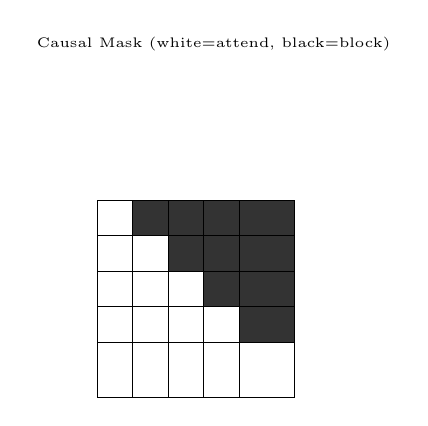
\begin{tikzpicture}[scale=0.45, every node/.style={font=\tiny}]
  \node at (2.5, 5.2) {Causal Mask (white=attend, black=block)};
  \foreach \i in {0,...,4} {
    \foreach \j in {0,...,4} {
      \pgfmathtruncatemacro{\val}{\j <= \i ? 1 : 0}
      \ifnum\val=1
        \node[draw, fill=white, minimum size=0.7cm] at (\j, -\i) {};
      \else
        \node[draw, fill=black!80, text=white, minimum size=0.7cm] at (\j, -\i) {};
      \fi
    }
  }
\end{tikzpicture}

The masked attention computation is:

\[
  \text{Attention}(Q, K, V) = \text{softmax}\!\left(\frac{QK^\top}{\sqrt{d_k}} + \text{mask}\right)V
\]

\begin{pseudocode}[Causal (Masked) Self-Attention]
def causal_self_attention(Q: Tensor, K: Tensor, V: Tensor) -> Tensor:
    # Q: [batch, seq_len, d_k], K: [batch, seq_len, d_k], V: [batch, seq_len, d_v]
    d_k = Q.size(-1)
    seq_len = Q.size(-2)
    scores = Q @ K.transpose(-2, -1)  # [batch, seq_len, d_k] @ [batch, d_k, seq_len] -> [batch, seq_len, seq_len]
    scaled_scores = scores / math.sqrt(d_k)  # [batch, seq_len, seq_len]
    # Create causal mask: upper triangle is True (positions to block)
    mask = torch.triu(torch.ones(seq_len, seq_len, dtype=torch.bool), diagonal=1)  # [seq_len, seq_len]
    scaled_scores = scaled_scores.masked_fill(mask, float('-inf'))  # [batch, seq_len, seq_len]
    attn_weights = softmax(scaled_scores, dim=-1)  # [batch, seq_len, seq_len]
    output = attn_weights @ V  # [batch, seq_len, seq_len] @ [batch, seq_len, d_v] -> [batch, seq_len, d_v]
    return output
\end{pseudocode}

\begin{keyconcept}
  We use \texttt{masked\_fill} to directly set blocked positions to
  $-\infty$ in the score matrix. This matters because the alternative---multiplying
  a 0/1 mask into the scores---would produce NaN when 0 is multiplied by
  $-\infty$: $0 \times (-\infty) = \text{NaN}$. The \texttt{masked\_fill}
  operation sidesteps this by never computing $0 \times (-\infty)$; it simply
  replaces the blocked positions with $-\infty$ before softmax is applied.
  Some implementations add the mask as an additive bias ($+\text{mask}$)
  where the mask contains $0$ for allowed positions and $-\infty$ for blocked
  positions---this is equivalent to \texttt{masked\_fill}.
\end{keyconcept}

\section{Multi-Head Attention}

A single attention head computes one set of attention weights, which means it
can learn only one pattern of relationships. In practice, language has many
kinds of relationships: grammatical subject--verb agreement, coreference
resolution, semantic relatedness, positional proximity, and more. Multi-head
attention addresses this by running $h$ parallel attention computations (``heads''),
each with its own Q/K/V projections, then concatenating and projecting the
results.

Instead of one large attention computation with dimension $d_{\text{model}}$,
multi-head attention splits the embedding dimension into $h$ heads of dimension
$d_k = d_{\text{model}} / h$. Each head can attend to different aspects of the
input independently. The outputs are concatenated and passed through a final
linear projection $W_O$ that lets heads interact and mix information.

The projection matrices have the following shapes:
\begin{itemize}
  \item $W_Q, W_K \in \mathbb{R}^{d_{\text{model}} \times d_k}$ (or $\mathbb{R}^{d_{\text{model}} \times d_{\text{model}}}$ when combined for all heads)
  \item $W_V \in \mathbb{R}^{d_{\text{model}} \times d_v}$ (usually $d_v = d_k$)
  \item $W_O \in \mathbb{R}^{d_{\text{model}} \times d_{\text{model}}}$ (projects concatenated heads back to embed dim)
\end{itemize}

\begin{pseudocode}[Multi-Head Attention]
def multi_head_attention(X: Tensor, n_heads: int) -> Tensor:
    # X: [batch, seq_len, embed_dim]
    # W_Q, W_K, W_V: [embed_dim, embed_dim], W_O: [embed_dim, embed_dim]
    batch, seq_len, embed_dim = X.shape
    d_k = embed_dim // n_heads

    # Project inputs to Q, K, V
    Q = X @ W_Q  # [batch, seq_len, embed_dim]
    K = X @ W_K  # [batch, seq_len, embed_dim]
    V = X @ W_V  # [batch, seq_len, embed_dim]

    # Reshape to separate heads: [batch, seq_len, embed_dim] -> [batch, n_heads, seq_len, d_k]
    Q = Q.view(batch, seq_len, n_heads, d_k).transpose(1, 2)
    K = K.view(batch, seq_len, n_heads, d_k).transpose(1, 2)
    V = V.view(batch, seq_len, n_heads, d_k).transpose(1, 2)

    # Compute attention for each head (in parallel via batched operations)
    # attn_output: [batch, n_heads, seq_len, d_k]
    attn_output = scaled_dot_product_attention(Q, K, V)

    # Concatenate heads: [batch, n_heads, seq_len, d_k] -> [batch, seq_len, embed_dim]
    attn_output = attn_output.transpose(1, 2).contiguous().view(batch, seq_len, embed_dim)

    # Final output projection lets heads interact
    output = attn_output @ W_O  # [batch, seq_len, embed_dim]
    return output
\end{pseudocode}

\begin{keyconcept}
  The reshaping pattern is the key to understanding multi-head attention:
  \begin{itemize}
    \item \textbf{Split}: $[\text{batch}, \text{seq}, \text{embed}] \rightarrow
          [\text{batch}, h, \text{seq}, d_k]$
    \item \textbf{Attend}: each head computes scaled dot-product attention
          independently
    \item \textbf{Concat}: $[\text{batch}, h, \text{seq}, d_k] \rightarrow
          [\text{batch}, \text{seq}, \text{embed}]$
  \end{itemize}
  The output projection $W_O$ is essential---without it, heads cannot
  interact and mix information. Removing $W_O$ would mean the concatenated
  heads are simply stacked side-by-side with no cross-head communication.
\end{keyconcept}

Why not just use a single head with a larger dimension? The answer is
expressiveness. With $h$ heads, each of dimension $d_k = d_{\text{model}}/h$,
the model learns $h$ different attention patterns in parallel. Empirically,
multi-head attention significantly outperforms single-head attention at the
same total dimensionality.

\section{Attention as Soft Dictionary Lookup}

The Q/K/V formulation can be understood through the lens of a \emph{soft
dictionary}: a differentiable generalization of a hash table or database
lookup. The database analogy from Section~2 applies here too, but now we can
see how it plays out \emph{across layers} of a deep network.

In a standard dictionary, the lookup returns exactly one value (hard match).
Attention returns a distribution over values (soft match). This softness is
what makes attention differentiable: the gradients flow through all
value contributions proportionally to their attention weights.

\begin{keyconcept}
  \textbf{Layer depth matters}: early layers tend to capture local
  syntactic patterns (e.g., attending to adjacent words), while later
  layers capture broader semantic relationships (e.g., resolving pronoun
  references across long distances). This progression emerges naturally
  from training---the model learns that local patterns are easiest to model
  first and gradually builds up to longer-range dependencies.
\end{keyconcept}

\section{\texorpdfstring{$O(n^2)$}{O(n²)} Complexity and Modern Solutions}

The attention matrix is $n \times n$, where $n$ is the sequence length. This
gives:
\begin{itemize}
  \item \textbf{Time}: $O(n^2 d)$ for computing attention scores (every pair of
        positions, each with a $d$-dimensional dot product)
  \item \textbf{Space}: $O(n^2)$ for storing the attention matrix
\end{itemize}

For a 128K-token context, that is approximately 16 billion entries per attention
matrix, multiplied by the number of layers and heads. This quadratic scaling is
the primary bottleneck for long-context models.

To put this in perspective: a single attention layer with $n = 128{,}000$ tokens
requires $\sim\!128000^2 = 16.4$ billion floating-point values for the attention
matrix alone, consuming about 64~GB of memory (in float32). With multiple layers
and heads, long-context inference becomes prohibitively expensive without
optimization.

Modern solutions include:

\begin{center}
\begin{tabular}{ll}
\toprule
\textbf{Technique} & \textbf{Effect} \\
\midrule
KV Cache & Avoids recomputing past K/V during generation \\
Grouped Query Attention (GQA) & Reduces KV head count \\
Flash Attention & IO-aware algorithm, same $O(n^2)$ but faster \\
Sliding Window Attention & Limits attention to local context of width $w$, reducing to $O(nw)$ \\
Linear Attention & Approximates softmax for $O(n)$ time and space \\
\bottomrule
\end{tabular}
\end{center}

\begin{keyconcept}
  \textbf{KV Cache} is perhaps the most impactful practical optimization.
  During autoregressive generation, each new token must attend to all previous
  tokens. Without caching, this means recomputing the keys and values for all
  previous positions at every step. With caching, the keys and values for
  previous positions are stored and only the new position's K/V are computed.
  This reduces the per-step cost from $O(n^2)$ to $O(n)$ during generation
  (though training still requires the full $O(n^2)$ computation).

  \textbf{Grouped Query Attention (GQA)} reduces the memory bottleneck by
  sharing keys and values across multiple query heads. Instead of $h$ separate
  KV pairs, GQA uses $g < h$ groups, each sharing one KV pair. This reduces
  the KV cache size by a factor of $h/g$.

  \textbf{Flash Attention} is an IO-aware algorithm that avoids materializing
  the full $n \times n$ attention matrix in GPU global memory. It computes
  attention in tiles, keeping partial results in faster SRAM. The algorithmic
  complexity remains $O(n^2)$, but the wall-clock time is dramatically
  reduced because it avoids the bottleneck of writing and reading the massive
  attention matrix from slow memory.

  \textbf{Sliding Window Attention} restricts each position to attend only to
  the $w$ most recent positions, reducing both time and space to $O(nw)$. This
  trades global context for efficiency; some models combine it with a few
  global attention tokens to retain long-range information.

  \textbf{Linear Attention} replaces the softmax with a kernel-based
  approximation $\text{sim}(q, k) = \phi(q)^\top \phi(k)$ that allows the
  computation to be reordered as $\phi(V)(\phi(K)^\top \phi(Q))$, eliminating
  the $n \times n$ matrix entirely. The result is $O(n)$ time and space, but
  the approximation quality is still an open research question.
\end{keyconcept}

The attention mechanism you have built in this chapter---scaled dot-product
attention with causal masking, organized into multiple heads---is the core
computational primitive of the transformer. The next chapter assembles this
primitive into a complete architecture: the GPT-2 model, wrapping attention
in residual connections, layer normalization, and feed-forward layers to form
the full transformer block.

\section*{Review Questions}

\begin{reviewquestion}[1]
  Why does scaled dot-product attention divide by $\sqrt{d_k}$ rather
  than $d_k$? What would happen with $\sqrt{d_k}$ omitted for a model
  with $d_k = 64$?
\end{reviewquestion}

\begin{reviewquestion}[2]
  Explain why the output projection $W_O$ in multi-head attention is
  necessary. What would happen if you removed it and just concatenated
  the heads?
\end{reviewquestion}

\begin{reviewquestion}[3]
  Consider a causal language model processing a 128K-token context.
  Assuming 12 layers and 12 heads per layer, how many $n \times n$
  attention matrices are computed during a single forward pass?
\end{reviewquestion}

\begin{reviewquestion}[4]
  Explain the difference between simplified self-attention and scaled
  dot-product attention. What do the learnable Q/K/V projections provide
  that raw embeddings cannot?
\end{reviewquestion}

\begin{reviewquestion}[5]
  In the causal mask, position $i$ is allowed to attend to position $j$
  when $j \leq i$. Why is the condition $j \leq i$ rather than $j < i$?
  What would happen if a position could not attend to itself?
\end{reviewquestion}

\begin{reviewquestion}[6]
  Using the database analogy, explain what the query, key, and value
  represent. Why is the result of attention a ``soft'' lookup rather
  than a ``hard'' lookup?
\end{reviewquestion}

\begin{reviewquestion}[7]
  Suppose you have a 6-token sequence and multi-head attention with
  3 heads and $d_{\text{model}} = 48$. What is the dimension of each
  head's Q, K, and V? What is the shape of the attention score matrix
  for a single head?
\end{reviewquestion}

\begin{reviewquestion}[8]
  Why does \texttt{masked\_fill} with $-\infty$ produce the correct
  causal mask, while multiplying by 0 could cause numerical issues?
  Explain with a concrete edge case.
\end{reviewquestion}

\begin{reviewquestion}[9]
  How does attention address the two main limitations of RNNs
  (sequential processing bottleneck and difficulty with long-range
  dependencies)?
\end{reviewquestion}

\begin{reviewquestion}[10]
  In multi-head attention, each head operates on dimension $d_k =
  d_{\text{model}} / h$. If you doubled the number of heads while
  keeping $d_{\text{model}}$ fixed, how would this affect the total
  number of parameters and the per-head computational cost?
\end{reviewquestion}

\begin{reviewquestion}[11]
  Explain how the KV cache works during autoregressive generation.
  Why does it reduce the per-step cost from $O(n^2)$ to $O(n)$?
\end{reviewquestion}

\begin{reviewquestion}[12]
  Grouped Query Attention (GQA) shares KV pairs across groups of query
  heads. Explain the tradeoff: what does GQA save, and what might it
  sacrifice?
\end{reviewquestion}

\begin{reviewquestion}[13]
  Why are three separate projection matrices ($W_Q$, $W_K$, $W_V$) used
  instead of a single shared projection? What capability would be lost
  if $W_K = W_V$?
\end{reviewquestion}

\begin{reviewquestion}[14]
  When implementing softmax from scratch, why must you subtract the
  maximum value before exponentiating? What would happen numerically
  with $d_k = 64$ and unscaled dot products if you skipped this step?
\end{reviewquestion}

\section*{Problems}

\begin{problem}[1]
  \textbf{Simplified Self-Attention from Scratch.}
  Implement simplified self-attention using only basic tensor operations
  (matrix multiplication and softmax---no \texttt{nn.Module} or learned
  parameters). Your function should take an input tensor of shape
  $[\text{batch}, \text{seq\_len}, \text{embed\_dim}]$ and return an output tensor of the
  same shape. Verify that each row of the attention weight matrix sums to 1.
\end{problem}

\begin{problem}[2]
  \textbf{Scaled Dot-Product Attention.}
  Implement scaled dot-product attention with learnable $W_Q$, $W_K$, $W_V$
  projections as \texttt{nn.Linear} modules. Write a function
  \texttt{scaled\_dot\_product\_attention(Q, K, V)} that computes
  $\text{softmax}(QK^\top / \sqrt{d_k})V$. Implement softmax from scratch
  (with max-subtraction for numerical stability) rather than using
  \texttt{torch.softmax}. Verify that removing the $\sqrt{d_k}$ scaling
  causes softmax to produce near-one-hot vectors for large $d_k$ (e.g.,
  $d_k = 256$).
\end{problem}

\begin{problem}[3]
  \textbf{Causal Masking.}
  Add causal masking to your scaled dot-product attention implementation.
  Create a boolean upper-triangular mask using \texttt{torch.triu} and
  apply it with \texttt{masked\_fill}. Feed a sequence of 8 tokens and
  verify that position $i$ in the output depends only on positions
  $0, 1, \ldots, i$ by checking that setting a future token to a
  different value does not change the output at position $i$.
\end{problem}

\begin{problem}[4]
  \textbf{Multi-Head Attention.}
  Implement multi-head attention by extending your single-head
  implementation. Use the reshape--transpose pattern to split the
  embedding dimension into $h$ heads, compute attention in parallel,
  and concatenate and project the result with $W_O$. Test with
  \texttt{embed\_dim = 48} and \texttt{n\_heads = 3}, verifying the
  output shape is $[\text{batch}, \text{seq\_len}, \text{embed\_dim}]$.
\end{problem}

\begin{problem}[5]
  \textbf{Attention Complexity Experiment.}
  Measure the wall-clock time of your multi-head attention implementation
  for sequence lengths $[128, 256, 512, 1024, 2048]$. Plot time vs.\
  sequence length. Does the empirical curve match the theoretical
  $O(n^2)$ prediction? How does the memory usage scale? Use
  \texttt{torch.cuda.max\_memory\_allocated()} if a GPU is available,
  or estimate memory from the size of the attention matrix.
\end{problem}
\chapter{The GPT Architecture}

\section{Token and Positional Embeddings}

Given a sequence of token IDs $[t_1, t_2, \ldots, t_n]$:

\[
  x_i = \text{Embed}_{\text{token}}(t_i) + \text{Embed}_{\text{pos}}(i)
\]

\begin{keyconcept}
  Token embeddings convert discrete IDs to continuous vectors.
  Positional embeddings give the model information about \emph{where}
  each token appears---without them, the model is permutation-invariant
  (bag-of-words).

  In GPT-2, both are learned \texttt{nn.Embedding} layers.
  The vocabulary size is 50,257 and the maximum context length is 1,024.
\end{keyconcept}

\section{LayerNorm and Residual Connections}

Each TransformerBlock uses \textbf{pre-norm} architecture:

\[
  \text{out} = x + \text{Dropout}\!\left(\text{Sublayer}\!\left(\text{LayerNorm}(x)\right)\right)
\]

\begin{keyconcept}
  \textbf{Why residual connections?} They provide a ``clean path'' for
  gradients to flow through deep networks:
  \[
    \frac{\partial}{\partial x}\bigl(x + f(x)\bigr) = 1 + \frac{\partial f}{\partial x}
  \]
  Even if $\frac{\partial f}{\partial x}$ is small, gradients can still
  flow through the $+1$ term, preventing vanishing gradients.
\end{keyconcept}

\section{Pre-Norm vs Post-Norm}

\begin{center}
\begin{tabular}{lll}
\toprule
 & \textbf{Pre-Norm (GPT-2+)} & \textbf{Post-Norm (Original)} \\
\midrule
Formula & $x + f(\text{LN}(x))$ & $\text{LN}(x + f(x))$ \\
LN position & Before sublayer & After sublayer \\
Gradient flow & LN \emph{not} in residual path & LN \emph{in} residual path \\
Training stability & Stable without warmup & Requires warmup \\
\bottomrule
\end{tabular}
\end{center}

\begin{keyconcept}
  In 12-layer networks, pre-norm produces gradients $\sim5\times$ larger
  at embedding layers compared to post-norm. This is because in
  post-norm, LayerNorm sits inside the residual path, and its gradients
  can shrink the signal flowing backward. Pre-norm keeps LayerNorm
  ``outside'' the residual path, preserving gradient magnitude.
\end{keyconcept}

\section{Feed-Forward Network}

The FFN in each block has two linear layers with a GELU activation:

\[
  \text{FFN}(x) = W_2\!\left(\text{GELU}(W_1 x + b_1)\right) + b_2
\]

where GELU is defined as:

\[
  \text{GELU}(x) = x \cdot \Phi(x) \approx 0.5\,x\left(1 + \tanh\!\left[\sqrt{\frac{2}{\pi}}\left(x + 0.044715x^3\right)\right]\right)
\]

\begin{keyconcept}
  The FFN's hidden dimension is typically $4\times$ the embedding
  dimension (e.g., 768 $\rightarrow$ 3072 for GPT-2 Small). This
  expansion allows the model to learn richer representations in a
  higher-dimensional space before projecting back down.
\end{keyconcept}

\section{Transformer Block Assembly}

A single TransformerBlock:

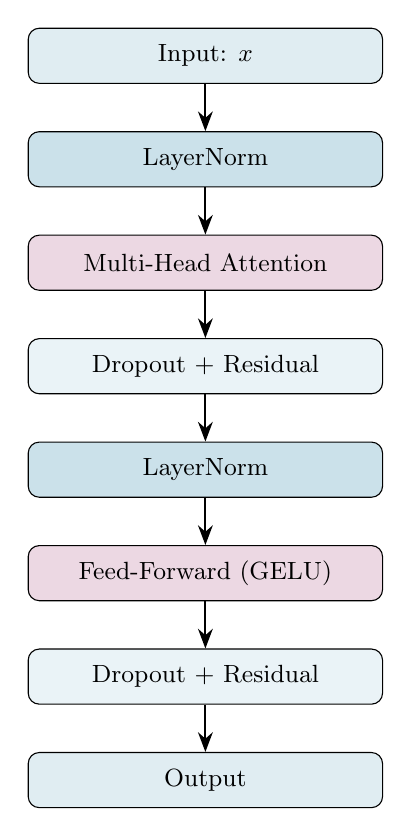
\begin{tikzpicture}[
  node distance=0.6cm,
  block/.style={rectangle, draw, rounded corners, minimum width=4.5cm,
                minimum height=0.7cm, font=\small},
  arrow/.style={-{Stealth[length=2.5mm]}, thick}
]
  \node[block, fill=accent!15] (input) {Input: $x$};
  \node[block, fill=accent!25, below=of input] (ln1) {LayerNorm};
  \node[block, fill=highlight!20, below=of ln1] (attn) {Multi-Head Attention};
  \node[block, fill=accent!10, below=of attn] (drop1) {Dropout + Residual};
  \node[block, fill=accent!25, below=of drop1] (ln2) {LayerNorm};
  \node[block, fill=highlight!20, below=of ln2] (ffn) {Feed-Forward (GELU)};
  \node[block, fill=accent!10, below=of ffn] (drop2) {Dropout + Residual};
  \node[block, fill=accent!15, below=of drop2] (output) {Output};

  \draw[arrow] (input) -- (ln1);
  \draw[arrow] (ln1) -- (attn);
  \draw[arrow] (attn) -- (drop1);
  \draw[arrow] (drop1) -- (ln2);
  \draw[arrow] (ln2) -- (ffn);
  \draw[arrow] (ffn) -- (drop2);
  \draw[arrow] (drop2) -- (output);
\end{tikzpicture}

Or more precisely:
\begin{align*}
  x' &= x + \text{Dropout}\!\left(\text{MHA}\!\left(\text{LN}_1(x)\right)\right) \\
  x'' &= x' + \text{Dropout}\!\left(\text{FFN}\!\left(\text{LN}_2(x')\right)\right)
\end{align*}

\section{Full GPT-2 Architecture}

Stack $N$ transformer blocks on top of embeddings, add a final
LayerNorm, and project to vocabulary-sized logits:

\begin{pseudocode}[GPT-2 Forward Pass]
$x \leftarrow \text{Embed}_{\text{token}}(\text{ids}) + \text{Embed}_{\text{pos}}(\text{positions})$\\[3pt]
\textbf{for} block $1$ \textbf{to} $N$:\\
\quad $x \leftarrow \text{TransformerBlock}(x)$ \hfill\textrm{\small (includes residual connections)}\\[3pt]
$x \leftarrow \text{LayerNorm}(x)$\\
$\text{logits} \leftarrow \text{Linear}(x)$ \hfill\textrm{\small (project to vocab size)}\\
\textbf{return} logits
\end{pseudocode}

\begin{center}
\begin{tabular}{lccc}
\toprule
\textbf{Model} & \textbf{Embed Dim} & \textbf{Layers} & \textbf{Heads} \\
\midrule
GPT-2 Small  & 768  & 12 & 12 \\
GPT-2 Medium & 1024 & 24 & 16 \\
GPT-2 Large  & 1280 & 36 & 20 \\
GPT-2 XL     & 1600 & 48 & 25 \\
\bottomrule
\end{tabular}
\end{center}

\section{Text Generation Strategies}

\begin{itemize}
  \item \textbf{Greedy}: pick $\text{argmax}$ at each step. Deterministic
        but prone to repetition.
  \item \textbf{Temperature}: scale logits by $T$ before softmax.
        $T<1$ makes the distribution sharper; $T>1$ makes it flatter.
        \[
          P(w_i) = \frac{\exp(\text{logit}_i / T)}{\sum_j \exp(\text{logit}_j / T)}
        \]
  \item \textbf{Top-$k$}: sample only from the $k$ highest-probability
        tokens. Filters out unlikely tokens while maintaining randomness.
  \item \textbf{Top-$p$} (nucleus sampling): sample from the smallest
        set of tokens whose cumulative probability exceeds $p$.
        More adaptive than top-$k$ since the pool size varies.
\end{itemize}

\section*{Review Questions}

\begin{reviewquestion}[1]
  Why does the GPT-2 architecture use pre-norm instead of post-norm?
  What specific problem does pre-norm solve?
\end{reviewquestion}

\begin{reviewquestion}[2]
  A TransformerBlock has two sublayers (attention and FFN), each wrapped
  in a residual connection and LayerNorm. Write out the full computation
  for both sublayers with pre-norm.
\end{reviewquestion}

\begin{reviewquestion}[3]
  Explain the difference between top-$k$ and top-$p$ sampling. In what
  situation would top-$p$ produce a different set of candidate tokens
  than top-$k$?
\end{reviewquestion}
\chapter{Pretraining}

\section{Cross-Entropy Loss for Next-Token Prediction}

The model outputs logits of shape $[\text{batch} \times \text{seq\_len},
\text{vocab\_size}]$. The target is the shifted token IDs of shape
$[\text{batch} \times \text{seq\_len}]$.

\[
  \mathcal{L} = -\frac{1}{N}\sum_{i=1}^{N} \log P(w_{i+1} \mid w_1, \ldots, w_i)
\]

\begin{keyconcept}
  Cross-entropy expects:
  \begin{itemize}
    \item \textbf{Input}: logits $[\text{batch} \times \text{seq}, \text{vocab}]$
    \item \textbf{Target}: integer class indices $[\text{batch} \times \text{seq}]$
  \end{itemize}
  The target is the input shifted by 1 position: ``The cat sat'' $\rightarrow$
  ``cat sat on''.
\end{keyconcept}

\section{Training Loop with AdamW}

\begin{pseudocode}[Training Loop]
\textbf{for} epoch $= 1$ \textbf{to} $E$:\\
\quad \textbf{for} batch \textbf{in} dataloader:\\
\quad\quad logits $\leftarrow$ model(batch.input)\\
\quad\quad loss $\leftarrow$ CrossEntropy(logits, batch.target)\\
\quad\quad loss.backward()\\
\quad\quad optimizer.step()\\
\quad\quad optimizer.zero\_grad()
\end{pseudocode}

\begin{keyconcept}
  \textbf{AdamW} decouples weight decay from the gradient update:
  \[
    \theta_{t+1} = \theta_t - \eta\left(\frac{\hat{m}_t}{\sqrt{\hat{v}_t} + \epsilon} + \lambda \theta_t\right)
  \]
  Typical hyperparameters: $\text{lr} = 3 \times 10^{-4}$,
  weight decay $= 0.01$, $\beta_1 = 0.9$, $\beta_2 = 0.999$.
\end{keyconcept}

\section{Learning Rate Scheduling}

The learning rate follows a \textbf{warmup + cosine decay} schedule:

\[
  \text{lr}(t) =
  \begin{cases}
    \text{max\_lr} \cdot \frac{t}{T_w} & \text{if } t \leq T_w \\[6pt]
    \text{min\_lr} + \frac{1}{2}(\text{max\_lr} - \text{min\_lr})
    \left(1 + \cos\!\left(\pi \cdot \frac{t - T_w}{T - T_w}\right)\right)
    & \text{if } t > T_w
  \end{cases}
\]

where $T_w$ is the number of warmup steps (typically 10\% of total) and
$T$ is the total number of training steps. $\text{min\_lr}$ is typically
$\text{max\_lr} / 10$.

\begin{keyconcept}
  \textbf{Warmup} prevents instability at the start of training when
  gradients are large and the model is randomly initialized. \textbf{Cosine
  decay} allows the learning rate to decrease smoothly, enabling
  finer parameter adjustments in later stages of training.
\end{keyconcept}

\section{Weight Initialization}

GPT-2 initializes weights from $\mathcal{N}(0, 0.02)$ for embeddings
and linear layers. This small standard deviation prevents early
training instability.

\section{Gradient Accumulation}

When batch size is limited by GPU memory, gradient accumulation
simulates larger batches:

\begin{pseudocode}[Gradient Accumulation]
\textbf{for} step $= 1$ \textbf{to} total\_steps:\\
\quad batch\_loss $\leftarrow$ model(batch)\\
\quad scaled\_loss $\leftarrow$ batch\_loss / grad\_accml\_steps\\
\quad scaled\_loss.backward() \hfill $\triangleright$ Accumulate gradients\\
\quad \textbf{if} step \% grad\_accml\_steps $== 0$:\\
\quad\quad optimizer.step()\\
\quad\quad optimizer.zero\_grad()
\end{pseudocode}

\begin{keyconcept}
  Dividing the loss by \texttt{grad\_accml\_steps} ensures that the
  effective gradient magnitude is the same as with a true large batch.
  Without this division, gradients would be too large by a factor of
  \texttt{grad\_accml\_steps}.
\end{keyconcept}

\section{Mixed Precision Training}

Using \texttt{torch.autocast} with \textbf{bfloat16} (or float16):

\begin{pseudocode}[Mixed Precision]
\textbf{with} autocast(device\_type="cuda", dtype=bfloat16):\\
\quad logits $\leftarrow$ model(batch)\\
\quad loss $\leftarrow$ criterion(logits, targets)\\[3pt]
loss.backward()\\
optimizer.step()
\end{pseudocode}

\begin{keyconcept}
  Mixed precision stores weights in float32 but computes forward/backward
  passes in bfloat16, halving memory usage and often doubling throughput
  on modern GPUs. Bfloat16 has the same dynamic range as float32 (8 exponent
  bits), avoiding the overflow/underflow issues of float16.
\end{keyconcept}

\section*{Review Questions}

\begin{reviewquestion}[1]
  Why does gradient accumulation divide the loss by the number of
  accumulation steps? What would happen to the effective learning rate
  without this division?
\end{reviewquestion}

\begin{reviewquestion}[2]
  Sketch the warmup + cosine decay learning rate curve. What happens if
  you skip warmup and start at max\_lr immediately?
\end{reviewquestion}

\begin{reviewquestion}[3]
  Why does bfloat16 have a wider dynamic range than float16? How many
  exponent bits does each format use?
\end{reviewquestion}
\chapter{Loading Pretrained Weights}

Training a large language model from scratch requires enormous computational
resources---hundreds of GPU-hours for even a modest model. Rather than
repeating this expensive process, we can load \emph{pretrained weights}:
parameters that have already been trained on massive text corpora and
published by other researchers. This practice, known as \textbf{transfer
learning}, lets us skip pretraining entirely and immediately use or
fine-tune a model that already understands language.

The most widely used repository for pretrained model weights is
\textbf{HuggingFace}, an open-source platform that hosts thousands of
models. OpenAI released the GPT-2 weights through HuggingFace, making them
accessible to anyone. The general workflow for loading pretrained weights
is:

\begin{enumerate}
  \item Identify the model architecture (e.g., GPT-2 Small with 12 layers,
        768-dimensional embeddings, 12 attention heads).
  \item Download the weight checkpoint from HuggingFace.
  \item Determine the mapping between the checkpoint's parameter names and
        the names in the target architecture.
  \item Handle any differences in how weights are stored (e.g.,
        transpositions, fused matrices).
  \item Assign the weights to the model, skipping any parameters that
        differ in shape or don't have a match.
\end{enumerate}

This chapter walks through each of these steps for GPT-2, explaining the
subtleties that arise when two implementations of the same architecture
store their parameters differently.

\section{Linear Layers and Weight Matrices}

Before diving into weight loading, we need to understand how linear
transformations are represented in neural networks and how their weights
are stored.

A \textbf{linear layer} (also called a fully connected or dense layer)
performs the transformation:
\[
  y = Wx + b
\]
where $x \in \mathbb{R}^{d_{\text{in}}}$ is the input vector,
$W \in \mathbb{R}^{d_{\text{out}} \times d_{\text{in}}}$ is the weight
matrix, and $b \in \mathbb{R}^{d_{\text{out}}}$ is the bias vector.

In PyTorch, \texttt{nn.Linear(in\_features, out\_features)} stores the
weight matrix as a tensor of shape
$[\text{out\_features}, \text{in\_features}]$. This convention comes from
the matrix multiplication $y = Wx$: the weight matrix has one row per
output dimension and one column per input dimension.

\begin{keyconcept}
  The two linear layers in the GPT-2 feed-forward network (FFN) serve
  different roles:
  \begin{itemize}
    \item \textbf{Expansion layer} ($W_1$, called \texttt{ff1}): maps from
          embedding dimension (768) to a hidden dimension (3072). This is a
          $4\times$ expansion that gives the model more capacity to learn
          complex features.
    \item \textbf{Projection layer} ($W_2$, called \texttt{ff2}): maps from
          hidden dimension (3072) back down to embedding dimension (768).
  \end{itemize}
  In GPT-2, the FFN computation is:
  $\text{FFN}(x) = W_2 \cdot \text{GELU}(W_1 x + b_1) + b_2$
\end{keyconcept}

Similarly, the multi-head attention mechanism uses four linear layers in
each transformer block:

\begin{keyconcept}
  Multi-head attention projects the input into three sets of vectors and
  then combines the result:
  \begin{itemize}
    \item $W_Q$ (\texttt{W\_q}): the \textbf{query} projection. Maps input
          from embedding dimension (768) to the total query dimension (768).
          Each attention head uses a 64-dimensional slice.
    \item $W_K$ (\texttt{W\_k}): the \textbf{key} projection. Same
          dimensions as $W_Q$. Keys represent ``what information I hold.''
    \item $W_V$ (\texttt{W\_v}): the \textbf{value} projection. Same
          dimensions. Values represent ``what content I provide when
          attended to.''
    \item $W_O$ (\texttt{W\_o}): the \textbf{output} projection. Maps from
          embedding dimension (768) back to embedding dimension (768),
          combining the outputs of all heads.
  \end{itemize}
  Each of $W_Q$, $W_K$, $W_V$ is stored as an \texttt{nn.Linear(768, 768)}
  with shape $[768, 768]$.
\end{keyconcept}

\section{Conv1D vs.\ Linear: Why the Transpose Matters}

HuggingFace's GPT-2 implementation uses \texttt{Conv1D} layers instead of
\texttt{nn.Linear}. Despite the name, \texttt{Conv1D} here does not
perform convolution---it is simply a linear layer that stores its weight
matrix in a \emph{transposed} layout compared to \texttt{nn.Linear}.

The key difference is in how each layer computes the forward pass:
\begin{itemize}
  \item \texttt{nn.Linear}: $y = x \cdot W^\top + b$, where
        $W$ has shape $[\text{out\_features}, \text{in\_features}]$.
  \item \texttt{Conv1D}: $y = x \cdot W + b$, where
        $W$ has shape $[\text{in\_features}, \text{out\_features}]$.
\end{itemize}

Both compute the same mathematical operation---a linear projection. The
difference is purely in storage layout:

\begin{center}
\begin{tabular}{lll}
\toprule
 & \textbf{HuggingFace (Conv1D)} & \textbf{Standard (nn.Linear)} \\
\midrule
Weight shape & $[\text{in\_features}, \text{out\_features}]$ & $[\text{out\_features}, \text{in\_features}]$ \\
Forward pass & $x \cdot W + b$ & $x \cdot W^\top + b$ \\
Transpose needed when loading? & Yes & No \\
\bottomrule
\end{tabular}
\end{center}

\begin{keyconcept}
  The Conv1D convention comes from early deep learning frameworks where
  a 1D convolution with kernel size 1 is mathematically equivalent to a
  linear layer. HuggingFace inherited this convention from the original
  OpenAI GPT-2 code release. When loading HuggingFace GPT-2 weights into a
  model that uses \texttt{nn.Linear}, every Conv1D weight must be
  transposed.
\end{keyconcept}

To see why the transpose is necessary, consider a concrete example. A
layer projecting from 768 to 3072 dimensions:
\begin{itemize}
  \item HuggingFace stores it as shape $[768, 3072]$.
  \item \texttt{nn.Linear(768, 3072)} expects shape $[3072, 768]$.
\end{itemize}
Loading the HuggingFace weight directly into \texttt{nn.Linear} would cause
a shape mismatch. The fix is to transpose:
\texttt{weight.data = hf\_weight.T}.

\section{Weight Mapping}

The GPT-2 model consists of an embedding layer, 12 transformer blocks, a
final layer norm, and a linear output projection (the LM head). Each
transformer block contains the attention sublayers ($W_Q$, $W_K$, $W_V$,
$W_O$) and the feed-forward sublayers ($W_1$, $W_2$), along with their
biases and layer norm parameters.

HuggingFace's naming convention differs from what a straightforward
implementation might use. The mapping below shows how each parameter in a
standard implementation corresponds to a parameter in the HuggingFace
checkpoint:

\begin{center}
\begin{tabular}{lll}
\toprule
\textbf{Component} & \textbf{Standard name} & \textbf{HuggingFace name} \\
\midrule
Token embedding & \texttt{embedding.token.weight} & \texttt{transformer.wte.weight} \\
Position embedding & \texttt{embedding.positional.weight} & \texttt{transformer.wpe.weight} \\
Query projection & \texttt{blocks[$i$].attn.W\_q.weight} & \texttt{h[$i$].attn.c\_attn.weight}[:, :768] \\
Key projection & \texttt{blocks[$i$].attn.W\_k.weight} & \texttt{h[$i$].attn.c\_attn.weight}[:, 768:1536] \\
Value projection & \texttt{blocks[$i$].attn.W\_v.weight} & \texttt{h[$i$].attn.c\_attn.weight}[:, 1536:] \\
Output projection & \texttt{blocks[$i$].attn.W\_o.weight} & \texttt{h[$i$].attn.c\_proj.weight} \\
FFN expansion & \texttt{blocks[$i$].ff.ff1.weight} & \texttt{h[$i$].mlp.c\_fc.weight} \\
FFN projection & \texttt{blocks[$i$].ff.ff2.weight} & \texttt{h[$i$].mlp.c\_proj.weight} \\
\bottomrule
\end{tabular}
\end{center}

There are two important differences beyond naming:

\subsection{Fused QKV Matrix}

HuggingFace stores the query, key, and value projections as a single fused
matrix:

\begin{keyconcept}
  HuggingFace combines $W_Q$, $W_K$, and $W_V$ into one
  \texttt{c\_attn} matrix of shape $[768, 2304]$. This is the
  concatenation of $W_Q$, $W_K$, and $W_V$ along the output dimension:
  \[
    \texttt{c\_attn.weight} = [W_Q \;||\; W_K \;||\; W_V]
  \]
  where each sub-matrix has shape $[768, 768]$ and $3 \times 768 = 2304$.
  To extract the individual projections, we split along the second axis.
\end{keyconcept}

\subsection{Transpositions}

Every weight listed in the table above comes from a \texttt{Conv1D} layer
in HuggingFace's implementation, which means every one of these weights
must be transposed when loading into an \texttt{nn.Linear}-based model.

\section{Loading the Weights}

Loading pretrained weights requires iterating through the checkpoint's
parameter names, matching each to the correct parameter in the target
model, and applying any necessary transformations (transpositions,
splits).

\begin{pseudocode}[Load HuggingFace GPT-2 Weights]
def load_gpt2_weights(model: GPTModel, hf_params: dict) -> None:
    # hf_params: flat dict mapping parameter names to tensors
    # Number of layers extracted from the checkpoint
    n_layers = hf_params["transformer.h.__0__"].shape  # or infer from keys
    for name, param in model.named_parameters():
        # Skip biases and layer norms for brevity
        # Match name patterns to HuggingFace equivalents
        if name == "embedding.token.weight":
            param.data = hf_params["transformer.wte.weight"]
        elif name == "embedding.positional.weight":
            param.data = hf_params["transformer.wpe.weight"]
        elif "attn.W_q" in name:
            # Slice columns 0:768 from the fused c_attn, then transpose
            # Shape: [768, 768] (after transpose) -> [768, 768]
            W_q = hf_params[hf_name][:, :768].T
            param.data = W_q
        elif "attn.W_k" in name:
            # Slice columns 768:1536 from the fused c_attn, then transpose
            W_k = hf_params[hf_name][:, 768:1536].T
            param.data = W_k
        elif "attn.W_v" in name:
            # Slice columns 1536: from the fused c_attn, then transpose
            W_v = hf_params[hf_name][:, 1536:].T
            param.data = W_v
        elif "attn.W_o" in name:
            # c_proj has shape [768, 768], transpose for nn.Linear
            param.data = hf_params[hf_name].T
        elif "ff.ff1" in name:
            # c_fc has shape [768, 3072], transpose for nn.Linear
            # After transpose: [3072, 768] matching nn.Linear(768, 3072)
            param.data = hf_params[hf_name].T
        elif "ff.ff2" in name:
            # c_proj has shape [3072, 768], transpose for nn.Linear
            # After transpose: [768, 3072] matching nn.Linear(3072, 768)
            param.data = hf_params[hf_name].T
\end{pseudocode}

\begin{keyconcept}
  The weight loading process involves three types of transformations:
  \begin{itemize}
    \item \textbf{Direct copy}: token and positional embeddings transfer
          directly with no transformation.
    \item \textbf{Transpose}: all linear and Conv1D weights require
          transposition because of the storage layout difference.
    \item \textbf{Split + transpose}: the fused QKV matrix must first be
          split into three slices along the output dimension, then each
          slice is transposed.
  \end{itemize}
\end{keyconcept}

A robust implementation should also handle parameters that don't have a
match---the final layer norm, biases, and any extra parameters should be
skipped with a warning rather than causing an error.

\section{Weight Tying}

In GPT-2, the token embedding matrix and the output projection (the
\emph{language model head}, or LM head) share the same weight tensor:

\[
  \texttt{lm\_head.weight} = \texttt{embedding.token.weight}
\]

This practice, called \textbf{weight tying} (or weight sharing), means the
same matrix is used for two different purposes:

\begin{enumerate}
  \item \textbf{At input}: mapping token IDs to embedding vectors (looking
        up rows of the matrix).
  \item \textbf{At output}: projecting the final hidden state to vocabulary
        logits (matrix multiplication with the hidden state).
\end{enumerate}

\begin{keyconcept}
  Weight tying saves approximately 38M parameters for GPT-2 Small
  (vocabulary size 50,257 $\times$ embedding dimension 768 $= 38,597,376$
  parameters, roughly one-third of the model's 124M total). Beyond saving
  memory, weight tying has a theoretical motivation: the same
  representations used to encode tokens should be useful for decoding them.
  If a token is embedded near certain vectors, the output projection should
  assign high probability to that same token when those vectors appear.
  This symmetry has been shown to improve model quality, especially in
  early training.
\end{keyconcept}

When loading HuggingFace weights, the LM head matrix does not appear as a
separate entry in the checkpoint---it is simply the token embedding matrix
reused. Any implementation must explicitly tie these weights:

\begin{pseudocode}[Weight Tying]
def tie_weights(model: GPTModel) -> None:
    # lm_head is a nn.Linear layer projecting from 768 to 50257
    # embedding.token is an nn.Embedding of shape [50257, 768]
    model.lm_head.weight = model.embedding.token.weight
    # Now both parameters point to the same underlying tensor
\end{pseudocode}

\section{Validating Loaded Weights}

After loading weights, it is crucial to verify that the model works
correctly. A model with improperly loaded weights---for example, if a
transposition was forgotten or if Q and V were swapped---will produce
gibberish rather than coherent text.

The simplest validation is to generate text from a known prompt and check
that the output is coherent:

\begin{pseudocode}[Validate Loaded Weights via Text Generation]
def validate_weights(model: GPTModel, tokenizer: Tokenizer) -> None:
    # The model should produce coherent English text
    prompt = "The capital of France is"
    token_ids = tokenizer.encode(prompt)
    # [batch, seq_len] = [1, 5]
    input_tensor = torch.tensor([token_ids])

    # Generate 20 new tokens using greedy decoding
    for _ in range(20):
        # logits shape: [1, seq_len, vocab_size]
        logits = model(input_tensor)
        # Take logits at the last position only
        next_token_id = logits[:, -1, :].argmax(dim=-1)  # [1]
        input_tensor = torch.cat([input_tensor, next_token_id.unsqueeze(1)], dim=1)

    output_text = tokenizer.decode(input_tensor[0])
    # Expected: coherent continuation like " Paris, which is the..."
    print(output_text)
\end{pseudocode}

\begin{keyconcept}
  \textbf{Common bugs when loading weights:}
  \begin{itemize}
    \item \textbf{Forgetting to transpose}: the model runs but produces
          gibberish because every linear layer computes $x \cdot W$ instead
          of $x \cdot W^\top$.
    \item \textbf{Swapping Q, K, V}: splitting the fused matrix incorrectly
          results in nonsensical attention patterns.
    \item \textbf{Missing weight tying}: the LM head uses random weights
          while the embedding uses pretrained weights, so the model cannot
          predict tokens correctly.
    \item \textbf{Shape mismatches}: silently assigning a wrong-shaped tensor
          (e.g., not splitting the fused QKV) causes dimension errors.
  \end{itemize}
\end{keyconcept}

Another useful check is to verify that the loaded parameters match the
expected shapes and have reasonable statistics (mean near zero, standard
deviation near 0.02 for GPT-2):

\begin{pseudocode}[Verify Weight Shapes and Statistics]
def verify_weights(model: GPTModel) -> None:
    for name, param in model.named_parameters():
        # Check shape matches expected dimensions
        print(f"{name}: shape={param.shape}")
        # GPT-2 weights initialized from N(0, 0.02)
        mean = param.data.mean().item()
        std = param.data.std().item()
        # Embedding weights have different scale; skip them
        if "embedding" not in name:
            assert abs(mean) < 0.01, f"{name} has suspicious mean: {mean}"
            # std should be close to 0.02 for trained weights
            assert 0.005 < std < 0.1, f"{name} has suspicious std: {std}"
\end{pseudocode}

\section{Perplexity Evaluation}

Once the pretrained weights are loaded and validated, we need a way to
quantitatively measure how well the model predicts text. The standard
metric for evaluating language models is \textbf{perplexity}.

\subsection{What Is Perplexity?}

Perplexity measures how ``surprised'' the model is by the text it sees. A
model that always assigns high probability to the correct next token has
low perplexity; a model that is frequently surprised has high perplexity.

Formally, given a sequence of tokens $w_1, w_2, \ldots, w_N$, the model
assigns each token a probability conditioned on the preceding tokens:
$P(w_i \mid w_1, \ldots, w_{i-1})$. Perplexity is defined as:

\[
  \text{Perplexity} = \exp\!\left(\frac{1}{N}\sum_{i=1}^{N} -\log P(w_i \mid w_{<i})\right)
  = \exp(\text{average cross-entropy loss per token})
\]

\begin{keyconcept}
  Perplexity can be interpreted as ``on average, how many tokens is the
  model equally uncertain about at each step.'' A perplexity of 30
  means the model is as uncertain as if it were choosing uniformly among
  30 tokens at each position.

  \textbf{Lower perplexity is better.} A perfect model that always assigns
  probability 1 to the correct next token would have perplexity 1. GPT-2
  Small achieves a perplexity around 30--40 on standard benchmarks like
  WikiText-103.
\end{keyconcept}

\subsection{Computing Perplexity}

Computing perplexity from a trained model involves three steps: tokenize
the evaluation text, run the model on the token sequences, and average the
cross-entropy loss across all tokens.

\begin{pseudocode}[Compute Perplexity]
def compute_perplexity(model: GPTModel, texts: list[str],
                       tokenizer: Tokenizer,
                       max_length: int = 1024) -> float:
    total_loss = 0.0
    total_tokens = 0
    for text in texts:
        # Tokenize and truncate to max_length
        token_ids = tokenizer.encode(text)[:max_length]
        # input: [seq_len] = [max_length]
        input_tensor = torch.tensor([token_ids])
        # targets: shifted by 1 position
        targets = input_tensor[:, 1:]   # [1, seq_len - 1]
        logits = model(input_tensor)[:, :-1, :]  # [1, seq_len - 1, vocab_size]

        # Cross-entropy loss averaged over tokens
        loss = cross_entropy(logits.reshape(-1, vocab_size),
                             targets.reshape(-1))
        total_loss += loss.item() * (len(token_ids) - 1)
        total_tokens += len(token_ids) - 1

    avg_loss = total_loss / total_tokens
    perplexity = math.exp(avg_loss)
    return perplexity
\end{pseudocode}

\begin{keyconcept}
  \textbf{Context length matters}: longer contexts give lower perplexity
  because the model has more information to condition on. Always compare
  perplexity at the same context length. A model evaluated with 1024-token
  contexts will appear better than the same model evaluated with 128-token
  contexts, even though the model itself is identical.
\end{keyconcept}

When computing perplexity, it is important to handle long texts properly.
The standard approach is to slide a window of length \texttt{max\_length}
across the text with some stride, computing loss only on the tokens that
fit within each window. This ensures every token is evaluated with the
maximum possible context.

\section*{Review Questions}

\begin{reviewquestion}[1]
  HuggingFace GPT-2 uses Conv1D with weight shape
  $[\text{in}, \text{out}]$ while PyTorch's \texttt{nn.Linear} uses
  $[\text{out}, \text{in}]$. What operation must you perform when
  loading weights?
\end{reviewquestion}

\begin{reviewquestion}[2]
  Explain weight tying between the token embedding and the LM head.
  Why does it make sense for these two matrices to share parameters?
\end{reviewquestion}

\begin{reviewquestion}[3]
  You evaluate the same model at context length 128 and context length
  1024. Which evaluation gives lower perplexity, and why?
\end{reviewquestion}

\begin{reviewquestion}[4]
  HuggingFace stores $W_Q$, $W_K$, and $W_V$ as a single fused matrix
  of shape $[768, 2304]$. How would you extract the individual weight
  matrices, and what is the shape of each after extraction?
\end{reviewquestion}

\begin{reviewquestion}[5]
  Suppose you forgot to transpose a Conv1D weight when loading it into an
  \texttt{nn.Linear} layer. Will the model crash, produce garbage, or
  produce slightly degraded output? Explain your reasoning.
\end{reviewquestion}

\begin{reviewquestion}[6]
  How many parameters does weight tying save for GPT-2 Small? Express
  your answer both as a count and as a fraction of total model parameters.
\end{reviewquestion}

\begin{reviewquestion}[7]
  Why does the GPT-2 FFN expand the hidden dimension from 768 to 3072
  before projecting back down? What would happen if the hidden dimension
  were equal to the embedding dimension (i.e., no expansion)?
\end{reviewquestion}

\begin{reviewquestion}[8]
  A model achieves a perplexity of 1.0 on a dataset. What does this mean
  about the model's predictions? Is this realistic in practice?
\end{reviewquestion}

\begin{reviewquestion}[9]
  You load GPT-2 weights but forget to tie the LM head weights to the
  embedding weights. The LM head is now using its randomly initialized
  weights. What will the model's output look like, and why?
\end{reviewquestion}

\begin{reviewquestion}[10]
  When computing perplexity on a long document, why is it insufficient to
  simply truncate the text to \texttt{max\_length}? Describe a better
  approach.
\end{reviewquestion}

\begin{reviewquestion}[11]
  The query, key, and value projections all map from 768 to 768
  dimensions. Could they share a single weight matrix? What would be the
  consequence?
\end{reviewquestion}

\begin{reviewquestion}[12]
  Why is Conv1D called ``Conv1D'' when it performs a linear (matrix
  multiplication) operation? What is the historical reason?
\end{reviewquestion}

\begin{reviewquestion}[13]
  Explain the mathematical relationship between cross-entropy loss and
  perplexity. If a model's average cross-entropy loss is 3.5, what is its
  perplexity?
\end{reviewquestion}

\section*{Problems}

\begin{problem}[1]
  Write a function \texttt{load\_gpt2\_weights(model, checkpoint\_path)} that
  loads GPT-2 weights from a HuggingFace checkpoint file
  (\texttt{.bin} or \texttt{.safetensors}). Your function should:
  (a) iterate through all parameters in the checkpoint,
  (b) match each to the correct parameter in the model,
  (c) apply the necessary transpositions for Conv1D weights, and
  (d) handle the fused QKV matrix by splitting it into three separate
  weight matrices. Print a summary of loaded vs.\ skipped parameters.
\end{problem}

\begin{problem}[2]
  Verify weight tying in a loaded GPT-2 model. Write code that:
  (a) loads the pretrained weights including weight tying,
  (b) checks that \texttt{model.lm\_head.weight} and
  \texttt{model.embedding.token.weight} point to the same tensor in memory
  (use \texttt{id()} or \texttt{torch.equal()}),
  (c) modifies one entry in the token embedding and verifies that the
  corresponding entry in the LM head also changes.
\end{problem}

\begin{problem}[3]
  Implement a perplexity evaluation function that processes an arbitrary
  text dataset. Use a sliding window approach with configurable stride.
  Compare the perplexity of a model with correctly loaded GPT-2 weights
  against the same model with randomly initialized weights. How many
  orders of magnitude different are the perplexities?
\end{problem}

\begin{problem}[4]
  Write a diagnostic function \texttt{diagnose\_weight\_loading(model)} that
  checks each layer of a loaded GPT-2 model for common loading errors:
  (a) verify that weight matrices have the expected shapes,
  (b) check that means are near zero and standard deviations are near 0.02,
  (c) detect any weights that are still at their random initialization
  (by checking if the standard deviation matches the initialization
  distribution rather than the pretrained distribution), and
  (d) generate a short text sample and print the first few predicted tokens
  to verify coherence.
\end{problem}

\begin{problem}[5]
  The fused QKV matrix in HuggingFace GPT-2 has shape $[768, 2304]$. Write
  a function that given this matrix, splits it into $W_Q$, $W_K$, and
  $W_V$, transposes each for use in \texttt{nn.Linear}, and assigns them
  to the corresponding model parameters. Then verify correctness by:
  (a) reconstructing the fused matrix from the individual weights and
  confirming it matches the original, and (b) checking that a forward pass
  through the attention layer produces the same output whether you use
  the fused or split weights.
\end{problem}
\chapter{Fine-Tuning}

Pretrained language models are impressively capable, but they are also
general-purpose: a model trained on internet-scale text can generate
plausible continuations for any prompt, but it cannot follow
instructions, answer questions, or classify sentiment out of the box.
Fine-tuning is the process of adapting a pretrained model to a specific
downstream task or behavior. In this chapter, we cover the core
techniques for fine-tuning: adding classification heads, instruction
fine-tuning with masked loss, attention masks, length-grouped batching,
gradient checkpointing, and parameter-efficient fine-tuning via LoRA.

\section{Classification Head}

Many NLP tasks can be framed as classification: sentiment analysis
(positive/negative), topic categorization, spam detection, and so on.
When adapting a language model for classification, we replace the
language-model head---which projects hidden states to vocabulary-sized
logits---with a smaller linear layer that maps to the number of
classes.

\subsection{From Next-Token Prediction to Classification}

During pretraining, the model learns rich representations of text. The
final hidden states encode semantic information that is useful far
beyond next-token prediction. For classification, we extract a single
vector from the sequence of hidden states and feed it into a
classification head:

\[
  \hat{y} = \text{softmax}\!\left(W_{\text{cls}} \cdot h_{\text{last}} + b_{\text{cls}}\right)
\]

where $h_{\text{last}} \in \mathbb{R}^{d_{\text{model}}}$ is the hidden
state at a chosen position, $W_{\text{cls}} \in \mathbb{R}^{n_{\text{classes}} \times d_{\text{model}}}$,
and $b_{\text{cls}} \in \mathbb{R}^{n_{\text{classes}}}$.

\begin{keyconcept}
  Why the last token? In causal (autoregressive) attention, every token
  can only attend to itself and preceding tokens. The last token has
  attended to \emph{all} preceding tokens, making its hidden state a
  summary of the entire sequence. This is analogous to the
  \texttt{[CLS]} token in BERT, but we don't need a special
  token---the last position naturally accumulates information from the
  full sequence.

  During pretraining, the model is trained so that the last token's
  hidden state predicts the next token given the entire context. This
  forces the last token to encode a compressed representation of
  everything it has seen, which transfers well to classification.
\end{keyconcept}

\begin{pseudocode}[Classification Forward Pass]
def classify(input_ids: Tensor,       # [batch, seq_len]
             model: GPTModel,
             cls_head: Linear,          # Linear(embed_dim, num_classes)
             pad_id: int) -> Tensor:    # [batch, seq_len]
    # Run full model to get hidden states
    hidden = model(input_ids)           # [batch, seq_len, embed_dim]

    # Find the last non-padding token for each sequence
    # attention_mask is 1 for real tokens, 0 for padding
    mask = (input_ids != pad_id)        # [batch, seq_len]
    # argmax finds the last True position (since seq is 0-indexed left-to-right)
    last_idx = mask.int().argmax(dim=1)  # [batch]
    # Gather the hidden state at the last real token
    last_hidden = hidden.gather(           # [batch, embed_dim]
        1, last_idx.unsqueeze(-1).expand(-1, hidden.size(-1))
    ).squeeze(1)
    # Classify
    logits = cls_head(last_hidden)        # [batch, num_classes]
    return logits
\end{pseudocode}

\begin{keyconcept}
  An important detail: when sequences are padded, we must extract the
  hidden state of the \emph{last real token}, not the last position in
  the tensor (which may be a padding token whose hidden state is
  meaningless). The code above uses the attention mask to locate this
  position.
\end{keyconcept}

\subsection{Training the Classification Head}

When fine-tuning for classification, there is a design choice: should
we update the pretrained weights, or freeze them and only train the
classification head?

\begin{itemize}
  \item \textbf{Frozen backbone}: Only $W_{\text{cls}}$ and
        $b_{\text{cls}}$ are updated. Works well when the pretrained
        model already encodes good features and the downstream task is
        simple. Also much faster and uses less memory.
  \item \textbf{Fine-tuning all weights}: The entire model is updated.
        Better for complex tasks that require adapting internal
        representations, but risks overfitting on small datasets and
        requires more memory.
  \item \textbf{Gradual unfreezing}: Start with a frozen backbone and
        progressively unfreeze layers from the top. A common compromise.
\end{itemize}

\section{Instruction Fine-Tuning and Masked Loss}

A pretrained language model generates text unconditionally---it does not
understand the concept of following instructions or engaging in
multi-turn conversation. Instruction fine-tuning teaches the model to
respond to structured prompts by training on examples formatted as
instruction--response pairs.

\subsection{Data Format}

Each training example is formatted as:

\begin{center}
\texttt{<prompt>Instruction here<|separator|>Response here<|eos|>}
\end{center}

The prompt portion provides context and instructions, and the response
is the desired output. During training, we want the model to learn to
\emph{generate the response}, not to copy the prompt. This means we
must compute loss only on the response tokens.

\subsection{Masked Targets}

PyTorch's \texttt{CrossEntropyLoss} supports an \texttt{ignore\_index}
parameter---any position in the target labeled with this index
contributes zero to the loss. By convention, \texttt{ignore\_index =
-100}. We set prompt tokens and padding tokens to $-100$ in the target
tensor:

\[
  \mathcal{L} = -\frac{1}{|\{i : t_i \neq -100\}|}\sum_{i:\, t_i \neq -100} \log P(t_i \mid \text{context})
\]

\begin{pseudocode}[Constructing Masked Targets for Instruction Fine-Tuning]
def build_masked_targets(input_ids: Tensor,       # [batch, seq_len]
                          prompt_lengths: Tensor,   # [batch]
                          pad_id: int,
                          eos_id: int) -> Tensor:   # [batch, seq_len]
    # Start with all positions masked
    targets = torch.full_like(input_ids, -100)  # [batch, seq_len]

    for i in range(input_ids.size(0)):
        prompt_len = prompt_lengths[i].item()
        # Copy response tokens (after prompt separator) into targets
        # Shift by 1: target at position t is the token at position t+1
        targets[i, prompt_len:-1] = input_ids[i, prompt_len + 1:]
        # Mask padding positions in the response
        # Find where real tokens end (excluding eos)
        response = input_ids[i, prompt_len:]
        real_len = (response != pad_id).sum().item()
        # Any remaining positions after real_len are already -100
        # and eos_id position is kept as a valid target

    # Also mask padding positions (where input_ids == pad_id)
    targets[input_ids == pad_id] = -100

    return targets  # [batch, seq_len] with -100 for prompt and padding
\end{pseudocode}

\begin{keyconcept}
  Padding tokens also use \texttt{ignore\_index = -100} so they don't
  contribute to loss. The \texttt{-100} value is PyTorch's convention
  for ``ignore this position.'' This is more memory-efficient than a
  separate binary mask because it reuses the target tensor itself.

  Two types of tokens are masked: (1) prompt tokens, because we don't
  want the model to learn to predict the user's instructions, and (2)
  padding tokens, because they carry no semantic content.
\end{keyconcept}

\section{Attention Masks}

When sequences in a batch have different lengths, shorter sequences are
padded to match the longest sequence in the batch. Attention masks tell
the model which positions contain real tokens and which are padding:

\begin{pseudocode}[Creating and Applying Attention Masks]
def apply_attention_mask(scores: Tensor,       # [batch, num_heads, seq_len, seq_len]
                          input_ids: Tensor,    # [batch, seq_len]
                          pad_id: int) -> Tensor:  # [batch, num_heads, seq_len, seq_len]
    # Create mask: True for real tokens, False for padding
    mask = (input_ids != pad_id)              # [batch, seq_len]

    # Expand mask for multi-head attention:
    # [batch, seq_len] -> [batch, 1, 1, seq_len]
    # Broadcasting will replicate across num_heads and query positions
    mask = mask.unsqueeze(1).unsqueeze(2)      # [batch, 1, 1, seq_len]

    # Apply: set padding positions to -inf before softmax
    # This makes padding tokens get zero attention weight
    scores = scores.masked_fill(~mask, float('-inf'))

    return scores  # [batch, num_heads, seq_len, seq_len]
\end{pseudocode}

\begin{keyconcept}
  The attention mask is expanded from $[\text{batch}, \text{seq}]$ to
  $[\text{batch}, 1, 1, \text{seq}]$ before being applied to the
  $[\text{batch}, \text{heads}, \text{seq}, \text{seq}]$ attention
  scores. Broadcasting replicates it across all heads and all query
  positions.

  During generation (autoregressive decoding), the attention mask must
  \emph{grow} alongside the token sequence---each newly generated token
  gets a mask value of 1 (real). This is handled by concatenating a new
  column of ones to the mask at each generation step.
\end{keyconcept}

\section{Length-Grouped Batching}

Instruction fine-tuning datasets contain sequences of widely varying
lengths. If we naively group random sequences into batches, each batch
must be padded to the length of its longest sequence. A batch containing
one sequence of 900 tokens and seven sequences of 50 tokens wastes
$850 \times 7 = 5{,}950$ padding positions.

\subsection{Grouping by Length}

The solution is to sort sequences by length (with added noise for
randomization) and then group similar-length sequences together into
batches. Short sequences go into one batch, long sequences into
another---each batch is padded only to its own maximum, not the global
maximum.

\begin{pseudocode}[Length-Grouped Batching]
def create_length_grouped_batches(
        examples: list[dict],          # Each has "input_ids" and "target"
        max_tokens: int,                # Max tokens per batch (GPU memory budget)
        noise_factor: float = 0.05      # Noise as fraction of max length
    ) -> list[list[dict]]:
    # Add noise to lengths for randomization within groups
    lengths = [len(ex["input_ids"]) for ex in examples]
    max_len = max(lengths)
    noisy_lengths = [
        l + int(noise_factor * max_len * random())
        for l in lengths
    ]
    # Sort by noisy length
    sorted_examples = sorted(
        zip(noisy_lengths, examples), key=lambda x: x[0]
    )
    examples = [ex for _, ex in sorted_examples]

    # Group into batches respecting token budget
    batches = []
    current_batch = []
    current_max_len = 0

    for ex in examples:
        seq_len = len(ex["input_ids"])
        # Check if adding this example would exceed token budget
        # New batch size * new max length must fit in budget
        new_max_len = max(current_max_len, seq_len)
        new_batch_size = len(current_batch) + 1
        if new_batch_size * new_max_len <= max_tokens:
            current_batch.append(ex)
            current_max_len = new_max_len
        else:
            batches.append(current_batch)
            current_batch = [ex]
            current_max_len = seq_len

    if current_batch:
        batches.append(current_batch)

    # Shuffle batch order to prevent length-biased gradient updates
    shuffle(batches)
    return batches
\end{pseudocode}

\begin{keyconcept}
  Without grouping: a batch containing sequences of length 900 and 50
  results in padding waste (all sequences padded to 900). With grouping,
  short and long sequences go into separate batches, minimizing padding.

  Dynamic batch sizing by token budget (not fixed batch size) is what
  actually prevents OOM: fewer long sequences per batch, more short
  ones. A batch of eight 50-token sequences uses 400 tokens, while a
  batch of two 900-token sequences uses 1{,}800 tokens---both fit within
  a 2{,}048-token budget, but with very different batch sizes.

  The noise factor prevents the model from seeing perfectly sorted data
  every epoch, which could introduce subtle biases.
\end{keyconcept}

\section{Gradient Checkpointing}

During the forward pass, a neural network computes intermediate
activations and stores them in memory for use during backpropagation.
For a Transformer with $L$ layers, these stored activations scale as
$O(L \cdot B \cdot S \cdot D)$, where $B$ is the batch size, $S$ is
the sequence length, and $D$ is the hidden dimension. For large models,
this activation memory can be the dominant memory cost---often larger
than the model weights themselves.

\subsection{How Checkpointing Works}

Gradient checkpointing reduces activation memory by not storing
intermediate activations for every layer. Instead, it stores only
``checkpoint'' activations at selected layer boundaries. During the
backward pass, when gradients are needed for a non-checkpointed layer,
the forward computation from the nearest checkpoint is re-executed to
recompute the required activations.

\begin{pseudocode}[Gradient Checkpointing for Transformer Blocks]
def forward_with_checkpointing(
        x: Tensor,                 # [batch, seq_len, embed_dim]
        blocks: list[TransformerBlock],
        checkpoint_segments: int = 3  # Number of checkpoint boundaries
    ) -> Tensor:
    # Divide blocks into segments; only store activations at boundaries
    blocks_per_segment = len(blocks) // checkpoint_segments

    # Forward pass with checkpointing
    for seg in range(checkpoint_segments):
        start = seg * blocks_per_segment
        end = start + blocks_per_segment
        segment_blocks = blocks[start:end]

        def run_segment(x: Tensor, seg_blocks=segment_blocks) -> Tensor:
            # This function will be re-run during backward if needed
            for block in seg_blocks:
                x = block(x)      # [batch, seq_len, embed_dim]
            return x

        # checkpoint() stores only the input x for this segment
        # During backward, it re-runs run_segment to recompute activations
        x = torch.utils.checkpoint.checkpoint(
            run_segment, x, use_reentrant=False
        )  # [batch, seq_len, embed_dim]

    # Process any remaining blocks (if not evenly divisible)
    for block in blocks[checkpoint_segments * blocks_per_segment:]:
        x = block(x)              # [batch, seq_len, embed_dim]

    return x
\end{pseudocode}

\begin{keyconcept}
  \textbf{Tradeoff}: Gradient checkpointing trades compute for memory.
  By recomputing activations during the backward pass, it saves
  $\sim$55--65\% of activation memory at the cost of $\sim$30\% slower
  training (due to the extra forward passes). On GPT-2 Large (36
  layers):

  \begin{center}
  73 GB $\rightarrow$ 33 GB ($\sim$55\% reduction)
  \end{center}

  The number of checkpoint segments controls the tradeoff: more segments
  means more recomputation but less memory. With a single checkpoint
  per layer (the finest granularity), memory scales as $O(\sqrt{L})$
  instead of $O(L)$. In practice, checkpointing every few layers is
  sufficient.
\end{keyconcept}

\section{LoRA (Low-Rank Adaptation)}

Fine-tuning all parameters of a large language model is expensive: the
full model must be loaded into memory, and optimizer states (Adam
maintains two additional tensors per parameter) can triple the memory
requirement. LoRA (Low-Rank Adaptation) is a parameter-efficient
fine-tuning method that freezes the original weights and adds small
trainable low-rank matrices, dramatically reducing the number of
trainable parameters while maintaining performance comparable to full
fine-tuning.

\subsection{The Low-Rank Decomposition}

LoRA applies a low-rank update to a pretrained weight matrix $W$. The
forward pass becomes:

\[
  h = Wx + \frac{\alpha}{r} BAx
\]

where:
\begin{itemize}
  \item $W \in \mathbb{R}^{d_{\text{out}} \times d_{\text{in}}}$ is the
        frozen pretrained weight matrix
  \item $B \in \mathbb{R}^{d_{\text{out}} \times r}$, initialized to zeros
  \item $A \in \mathbb{R}^{r \times d_{\text{in}}}$, initialized from
        $\mathcal{N}(0, \sigma^2)$ where $\sigma = 0.02$
  \item $r \ll d_{\text{in}}, d_{\text{out}}$ is the LoRA rank
  \item $\alpha$ is the scaling factor; effective scaling is $\alpha / r$
\end{itemize}

\subsection{Why Low Rank Works: A Concrete Example}

Consider a weight matrix $W \in \mathbb{R}^{768 \times 768}$ from
GPT-2 Small, with a LoRA rank of $r = 4$:

\begin{center}
\begin{tabular}{lrr}
\toprule
\textbf{Parameter} & \textbf{Shape} & \textbf{Count} \\
\midrule
$W$ (frozen) & $768 \times 768$ & 589{,}824 \\
$A$ (trainable) & $4 \times 768$ & 3{,}072 \\
$B$ (trainable) & $768 \times 4$ & 3{,}072 \\
LoRA update ($BA$) & $768 \times 768$ (implicit) & --- \\
\bottomrule
\end{tabular}
\end{center}

The update $BA$ produces a $768 \times 768$ matrix, but it is
constrained to lie in a 4-dimensional subspace---it has rank at most 4.
The full matrix $W$ has rank 768 (typically), so the LoRA update can
only modify the output along 4 directions. Yet this is enough: the
pretrained model is already close to a good solution, and fine-tuning
requires only small adjustments that tend to be low-rank.

The parameter savings are stark: 6{,}144 trainable parameters for the
LoRA adapter versus 589{,}824 for full fine-tuning of this single
matrix---a $\sim$96$\times$ reduction. Across all attention weight
matrices in GPT-2 Small (12 layers $\times$ 4 matrices each), the
total LoRA parameters are roughly 294K versus 780M for full
fine-tuning.

\subsection{Forward Pass}

\begin{pseudocode}[LoRA Linear Layer Forward Pass]
class LoRALinear(nn.Module):
    def __init__(self, in_dim: int, out_dim: int, rank: int, alpha: float):
        super().__init__()
        # Frozen pretrained weight
        self.W = nn.Linear(in_dim, out_dim, bias=False)
        self.W.weight.requires_grad_(False)

        # LoRA low-rank matrices
        self.lora_A = nn.Parameter(torch.randn(rank, in_dim) * 0.02)
        self.lora_B = nn.Parameter(torch.zeros(out_dim, rank))
        self.scaling = alpha / rank

    def forward(self, x: Tensor) -> Tensor:  # x: [batch, seq_len, in_dim]
        # Pretrained path (frozen)
        h_pretrained = self.W(x)              # [batch, seq_len, out_dim]

        # LoRA path: x -> A -> B (low-rank bottleneck)
        # Process sequence dimension with matrix operations
        h_lora = x @ self.lora_A.T             # [batch, seq_len, rank]
        h_lora = h_lora @ self.lora_B.T         # [batch, seq_len, out_dim]

        # Combine with scaling
        return h_pretrained + self.scaling * h_lora  # [batch, seq_len, out_dim]
\end{pseudocode}

\begin{keyconcept}
  \textbf{Why $B$ is zero-initialized}: At the start of fine-tuning,
  $BA = 0$ so $h = Wx$, meaning the model behaves exactly like the
  pretrained model. The LoRA update grows from zero, ensuring a smooth
  transition from the pretrained model's behavior.

  If $B$ were randomly initialized, the initial output would be $h =
  Wx + \frac{\alpha}{r}BAx$, introducing a large random perturbation
  that could destabilize training and temporarily degrade the model's
  capabilities.

  \textbf{Practical impact}: LoRA reduces trainable parameters from
  $\sim$780M to $\sim$6M on GPT-2 Large. The main savings come from
  eliminating optimizer states (Adam stores 2 extra tensors per
  parameter) and gradients for frozen weights. With LoRA, optimizer
  state memory scales with the number of \emph{trainable} parameters,
  not the total model size.

  \textbf{Merging for deployment}: At inference time, the LoRA weights
  can be merged into the original weights: $W' = W + \frac{\alpha}{r}
  BA$. After merging, there is no additional cost compared to a fully
  fine-tuned model---same latency, same memory.
\end{keyconcept}

\subsection{Which Layers to Apply LoRA To}

LoRA is typically applied to the attention weight matrices ($W_Q$,
$W_K$, $W_V$, $W_O$) and sometimes the feed-forward layers. Empirical
results show that:

\begin{itemize}
  \item Applying LoRA to all four attention matrices ($W_Q, W_K, W_V,
        W_O$) generally outperforms applying it to only $W_Q$ and
        $W_V$.
  \item Applying LoRA to feed-forward layers in addition to attention
        brings marginal improvement at the cost of more parameters.
  \item The rank $r$ is typically set between 4 and 64. Ranks of 8--16
        often provide a good balance between expressiveness and
        efficiency for instruction fine-tuning.
\end{itemize}

\section*{Review Questions}

\begin{reviewquestion}[1]
  Why does instruction fine-tuning use \texttt{ignore\_index = -100}
  instead of a separate mask tensor? What are the two types of tokens
  that should be masked out?
\end{reviewquestion}

\begin{reviewquestion}[2]
  Explain how length-grouped batching reduces padding waste. Why do
  we add noise to sequence lengths before sorting?
\end{reviewquestion}

\begin{reviewquestion}[3]
  LoRA initializes $B$ to zeros. Explain why this is important for
  fine-tuning. What would happen if $B$ were randomly initialized
  instead?
\end{reviewquestion}

\begin{reviewquestion}[4]
  In classification fine-tuning, why do we extract the hidden state of
  the last real token rather than the last position in the tensor? What
  would happen if we used the last position in a padded sequence?
\end{reviewquestion}

\begin{reviewquestion}[5]
  Explain the tradeoff made by gradient checkpointing. If you
  checkpoint every $k$ layers in a 24-layer model, approximately how
  many times is each layer's forward pass executed during one training
  iteration?
\end{reviewquestion}

\begin{reviewquestion}[6]
  For a $1024 \times 768$ weight matrix with LoRA rank $r = 8$ and
  $\alpha = 16$, compute the number of trainable parameters in the LoRA
  adapter. What is the effective scaling factor $\alpha / r$?
\end{reviewquestion}

\begin{reviewquestion}[7]
  Why does causal attention make the last token's hidden state a good
  representation for classification? Contrast this with BERT-style
  bidirectional attention.
\end{reviewquestion}

\begin{reviewquestion}[8]
  When building masked targets for instruction fine-tuning, the targets
  are shifted by one position relative to the input. Explain why this
  shift is necessary.
\end{reviewquestion}

\begin{reviewquestion}[9]
  Describe how dynamic batch sizing based on a token budget prevents
  out-of-memory errors during fine-tuning. Why can't we just use a
  fixed batch size?
\end{reviewquestion}

\begin{reviewquestion}[10]
  After LoRA fine-tuning, we can merge the LoRA weights into the
  original weights via $W' = W + \frac{\alpha}{r}BA$. What is the
  advantage of merging at deployment time? Is there any difference in
  inference latency between merged and unmerged LoRA?
\end{reviewquestion}

\begin{reviewquestion}[11]
  Gradient checkpointing reduces memory from $O(L)$ to $O(\sqrt{L})$
  for $L$ layers (with per-layer checkpointing). Derive why the memory
  scales as $O(\sqrt{L})$ when every layer is a checkpoint boundary.
\end{reviewquestion}

\begin{reviewquestion}[12]
  In the LoRA forward pass, the computation goes through a bottleneck:
  $x \to A \to B \to$ output, where $A$ is $r \times d_{\text{in}}$
  and $B$ is $d_{\text{out}} \times r$. Explain why the rank $r$
  controls the expressiveness of the LoRA update. What happens as $r
  \to d_{\text{in}}$?
\end{reviewquestion}

\section*{Problems}

\begin{problem}[1]
  \textbf{Implement a classification fine-tuning loop.} Given a
  pretrained GPT model, a classification head
  (\texttt{nn.Linear(embed\_dim, num\_classes)}), and a dataset of
  (text, label) pairs, implement the training loop that:
  (a) extracts the last real token's hidden state, (b) computes
  classification loss, (c) optionally freezes the backbone. Compare
  validation accuracy with a frozen backbone vs.\ fine-tuning all
  weights on a binary sentiment classification task.
\end{problem}

\begin{problem}[2]
  \textbf{Implement masked targets for instruction fine-tuning.}
  Write a function that takes a batch of tokenized instruction--response
  pairs (with a separator token and padding) and returns the target
  tensor with prompt and padding positions set to $-100$. Verify your
  implementation by checking that: (a) the loss on a batch equals the
  loss computed only on response tokens, and (b) padding tokens
  contribute zero to the loss.
\end{problem}

\begin{problem}[3]
  \textbf{Implement LoRA adapter layers.} Create a
  \texttt{LoRALinear} module that wraps an existing \texttt{nn.Linear}
  layer and adds the low-rank $A$ and $B$ matrices with configurable
  rank $r$ and scaling $\alpha$. Replace the attention weight matrices
  in a GPT model with LoRA-wrapped versions. Verify that at
  initialization, the LoRA model produces identical outputs to the
  original model (since $B$ is zero-initialized).
\end{problem}

\begin{problem}[4]
  \textbf{Implement length-grouped batching.} Given a list of
  tokenized sequences of varying lengths, implement a dataloader that
  sorts sequences by length (with a noise factor), groups them into
  batches respecting a maximum token budget, and pads each batch to its
  own maximum length. Measure the average padding waste per batch
  compared to random batching.
\end{problem}

\begin{problem}[5]
  \textbf{Implement gradient checkpointing.} Wrap each
  \texttt{TransformerBlock} in a GPT model with
  \texttt{torch.utils.checkpoint.checkpoint()} and measure: (a) peak
  GPU memory with and without checkpointing, (b) training throughput
  (tokens per second) with and without checkpointing. Report the
  memory savings and the throughput reduction.
\end{problem}
\chapter{Modern Architecture Deep Dives}

\section{RMSNorm}

RMSNorm simplifies LayerNorm by removing mean subtraction and bias:

\begin{align*}
  \textbf{LayerNorm:} \quad & \hat{x}_i = \frac{x_i - \mu}{\sqrt{\sigma^2 + \epsilon}}, \quad y_i = \gamma \hat{x}_i + \beta \\[6pt]
  \textbf{RMSNorm:} \quad & \hat{x}_i = \frac{x_i}{\sqrt{\frac{1}{d}\sum_{j=1}^{d} x_j^2 + \epsilon}}, \quad y_i = \gamma \hat{x}_i
\end{align*}

Key differences:
\begin{itemize}
  \item RMSNorm removes \textbf{mean subtraction}: it only rescales, not
        recenters
  \item RMSNorm has \textbf{no bias} parameter ($\beta$), only a gain
        $\gamma$
  \item In practice, negligible speed difference---normalization is a
        tiny fraction of total compute
\end{itemize}

\begin{keyconcept}
  \textbf{Float32 upcasting}: Both LayerNorm and RMSNorm must upcast to
  float32 before computing mean/variance/RMS. Low-precision types (bf16,
  fp16) can overflow or lose precision in these reduction operations.
  After computing the normalization in float32, the result is cast back
  to the original dtype before the affine transform.
\end{keyconcept}

\section{RoPE (Rotary Positional Embeddings)}

RoPE encodes position by \emph{rotating} pairs of dimensions in the
query and key vectors, rather than adding positional embeddings.

\subsection{The Key Idea}

For each pair of dimensions $(2i, 2i+1)$ at position $m$:

\[
  \begin{bmatrix} q_{2i}' \\ q_{2i+1}' \end{bmatrix}
  =
  \begin{bmatrix} \cos(m\theta_i) & -\sin(m\theta_i) \\ \sin(m\theta_i) & \cos(m\theta_i) \end{bmatrix}
  \begin{bmatrix} q_{2i} \\ q_{2i+1} \end{bmatrix}
\]

where $\theta_i = \frac{1}{\text{base}^{2i/d}}$ (base = 10000 by
default).

This is a 2D rotation by angle $m\theta_i$.

\subsection{Efficient Implementation: Rotate-and-Interleave}

Instead of handling pairs explicitly, we use the identity:

\[
  q' = q \odot \cos(m\boldsymbol{\theta}) + \text{rotate\_half}(q) \odot \sin(m\boldsymbol{\theta})
\]

where $\text{rotate\_half}$ constructs $(-q_{2i+1}, q_{2i})$ for each
pair, then interleaves. In code:

\begin{pseudocode}[Apply Rotary Embedding]
Reshape $x$ to $[\ldots, d/2, 2]$ \hfill\textrm{\small (pair up dimensions)}\\
$x_{\text{rot}} \leftarrow$ stack $(-x[\ldots, 1], x[\ldots, 0])$ along last dim\\
$x_{\text{rot}} \leftarrow$ flatten $x_{\text{rot}}$ \hfill\textrm{\small (interleave back)}\\
\textbf{return} $x \odot \cos + x_{\text{rot}} \odot \sin$
\end{pseudocode}

\begin{keyconcept}
  \textbf{Critical property}: With RoPE, the dot product
  $q_m^\top k_n$ depends \emph{only on the relative distance} $(m - n)$,
  not on absolute positions. This is because the rotation angle for $q$
  at position $m$ minus the rotation angle for $k$ at position $n$ equals
  the angle for relative position $(m-n)$.

  \textbf{RoPE is applied only to Q and K, never to V}. Position
  information enters exclusively through attention scores.
\end{keyconcept}

\section{SwiGLU}

SwiGLU replaces the standard GELU FFN with a gated architecture:

\begin{align*}
  \textbf{GELU FFN:} & \quad \text{FFN}(x) = W_2\!\left(\text{GELU}(W_1 x)\right) \\[4pt]
  \textbf{SwiGLU:} & \quad \text{FFN}(x) = W_{\text{down}}\!\left(W_{\text{gate}}(x) \odot \text{SiLU}(W_{\text{up}}(x))\right)
\end{align*}

where $\text{SiLU}(x) = x \cdot \sigma(x)$ (also called ``swish'').

\begin{keyconcept}
  \textbf{Key differences from standard FFN}:
  \begin{itemize}
    \item 3 linear layers instead of 2 ($W_{\text{gate}}$,
          $W_{\text{up}}$, $W_{\text{down}}$)
    \item The gate controls which features pass through: when
          $\text{SiLU}(W_{\text{up}}(x)) \approx 0$, the gate ``closes''
          and blocks information
    \item Despite having more parameters per layer, SwiGLU is
          empirically more parameter-efficient---it matches or exceeds
          GELU FFN quality with fewer total parameters
  \end{itemize}

  LLaMA compensates for the extra projection by using
  $d_{\text{ff}} = \frac{2}{3} \cdot 4d_{\text{model}}$ instead of
  $4d_{\text{model}}$; our implementation keeps $4d_{\text{model}}$
  for simplicity.
\end{keyconcept}

\section{\texorpdfstring{GQA}{GQA} (Grouped Query Attention)}

GQA reduces the KV cache by sharing KV heads across groups of query
heads:

\begin{center}
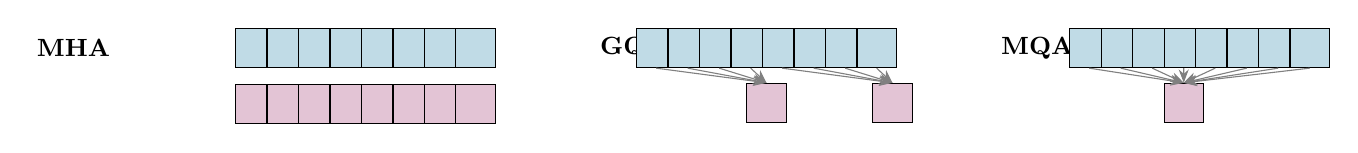
\begin{tikzpicture}[
  node distance=0.3cm and 0.8cm,
  qnode/.style={rectangle, draw, fill=accent!30, minimum width=0.5cm, minimum height=0.5cm, font=\tiny},
  kvnode/.style={rectangle, draw, fill=highlight!30, minimum width=0.5cm, minimum height=0.5cm, font=\tiny},
  label/.style={font=\small\bfseries}
]
 
  \node[label] (mhlabel) {MHA};
  \foreach \i in {1,...,8} {
    \node[qnode, right=0.15cm of mhlabel] (q\i) at ({1.5+\i*0.4}, 0) {};
    \node[kvnode, below=0.2cm of q\i] {};
  }
  
  \node[label, right=1.2cm of q8] (gqlabel) {GQA};
  \foreach \i in {1,...,8} {
    \node[qnode] (gq\i) at ({7+\i*0.4}, 0) {};
  }
  \foreach \i in {1,2} { \node[kvnode] (gkv\i) at ({7.2+\i*1.6}, -0.7) {}; }
  \draw[-{Stealth}, gray] (gq1.south) -- (gkv1.north);
  \draw[-{Stealth}, gray] (gq2.south) -- (gkv1.north);
  \draw[-{Stealth}, gray] (gq3.south) -- (gkv1.north);
  \draw[-{Stealth}, gray] (gq4.south) -- (gkv1.north);
  \draw[-{Stealth}, gray] (gq5.south) -- (gkv2.north);
  \draw[-{Stealth}, gray] (gq6.south) -- (gkv2.north);
  \draw[-{Stealth}, gray] (gq7.south) -- (gkv2.north);
  \draw[-{Stealth}, gray] (gq8.south) -- (gkv2.north);
  
  \node[label, right=1.2cm of gq8] (mqlabel) {MQA};
  \foreach \i in {1,...,8} {
    \node[qnode] (mq\i) at ({12.5+\i*0.4}, 0) {};
  }
  \node[kvnode] (mkv) at ({14.1}, -0.7) {};
  \foreach \i in {1,...,8} {
    \draw[-{Stealth}, gray] (mq\i.south) -- (mkv.north);
  }
\end{tikzpicture}
\end{center}

\begin{center}
\begin{tabular}{lccc}
\toprule
 & \textbf{MHA} & \textbf{GQA} & \textbf{MQA} \\
\midrule
Query heads & $h$ & $h$ & $h$ \\
KV heads & $h$ & $h_{\text{kv}} < h$ & 1 \\
Group size & 1 & $h / h_{\text{kv}}$ & $h$ \\
KV cache savings & None & $\times\, h_{\text{kv}}/h$ & $\times\, 1/h$ \\
\bottomrule
\end{tabular}
\end{center}

\begin{keyconcept}
  \textbf{Implementation}: After computing K and V with the smaller
  $W_K$ and $W_V$ matrices ($d_{\text{model}} \rightarrow h_{\text{kv}}
  \cdot d_k$), we expand them using
  \texttt{repeat\_interleave} to match the number of query heads:

  \begin{enumerate}
    \item Compute K, V with reduced projection: $[b, s, h_{\text{kv}} \cdot d_k]$
    \item Reshape: $[b, s, h_{\text{kv}}, d_k]$
    \item Transpose: $[b, h_{\text{kv}}, s, d_k]$
    \item Expand: $[b, h, s, d_k]$ via \texttt{repeat\_interleave}
  \end{enumerate}

  RoPE is applied \emph{after} KV expansion to avoid subtle numerical
  issues. The special cases: $h_{\text{kv}} = h$ gives standard MHA,
  $h_{\text{kv}} = 1$ gives Multi-Query Attention (MQA).
\end{keyconcept}

\section*{Review Questions}

\begin{reviewquestion}[1]
  RMSNorm removes both mean subtraction and the bias parameter compared
  to LayerNorm. What is the intuition for why removing mean subtraction
  still works well?
\end{reviewquestion}

\begin{reviewquestion}[2]
  Prove that with RoPE, the dot product $q_m^\top k_n$ depends only on
  the relative position $(m - n)$, not on absolute positions $m$ and $n$
  individually. (Hint: use the 2D rotation formulation.)
\end{reviewquestion}

\begin{reviewquestion}[3]
  Consider a model with 32 query heads and 4 KV heads using GQA.
  During autoregressive generation, how much smaller is the KV cache
  compared to standard MHA? At what cost?
\end{reviewquestion}

\end{document}